\documentclass[11pt,reqno,a4paper]{article}

\usepackage{graphicx} % Required for inserting images

\usepackage[toc,page]{appendix} % For appendix

%\usepackage[margin=4cm]{geometry} 

\usepackage{titling}  % For more control over title elements

% for bibliography
\usepackage[doi=true,isbn=false,style=alphabetic,sorting=none,backend=biber,maxnames=5,maxalphanames=5,giveninits=true]{biblatex}
\AtEveryBibitem{\clearlist{language}}
\bibliography{main}

% To make references look nice (has to be at the top):
\usepackage[breaklinks,plainpages,hypertexnames=false,plainpages=false]{hyperref}
\hypersetup{urlcolor=blue, citecolor=blue, linkcolor=blue}



% Must-haves for math:
\usepackage{amsmath} 
\usepackage{amsthm}
\usepackage{amssymb}
\usepackage{amsfonts}
\usepackage{dsfont}

\usepackage{tikz}
\usepackage{tikz-3dplot}
\usetikzlibrary{shapes.arrows}
\usetikzlibrary{arrows.meta}



\usepackage[capitalise, noabbrev]{cleveref} % for \cref

\usepackage{xcolor} % For color customization

\usepackage[cache=false]{minted} % Main minted package
\usemintedstyle{tango} % or try 'monokai', 'tango', 'pastie', etc.
\usepackage{adjustbox}
\usepackage{fvextra}
\usepackage[labelfont=bf]{caption} % Bold captions 

\usepackage{enumitem}


% For algorithms:
\usepackage[noend]{algorithmic} % for the algorithmic environment
\renewcommand{\algorithmicrequire}{\textbf{Input:}}
\renewcommand{\algorithmicensure}{\textbf{Output:}}

%\renewcommand{\baselinestretch}{1.1} % increases the space between lines


%%%%%%%%%%%%%%%%%%%%%%%%
%%%% Page settings %%%%%
%%%%%%%%%%%%%%%%%%%%%%%%
\setlength{\parindent}{0pt}
\setlength{\parskip}{6pt}
\renewcommand{\baselinestretch}{1.1}
%\setlength{\oddsidemargin}{-1in} % Linker Rand 30mm vom Papierrand
%\addtolength{\oddsidemargin}{30mm}
%\setlength{\evensidemargin}{\oddsidemargin}
%\setlength{\textwidth}{150mm} % Rechter Rand 30mm vom Papierrand



%%%%%%%%%%%%%%%%%%%%%%%%%%%%%%%%%
%%%% Begin Theorem Section  %%%%%
%%%%%%%%%%%%%%%%%%%%%%%%%%%%%%%%%
\newtheoremstyle{theoremstyle}
{10pt}      %  Space above
{5pt}       %  Space below
{\itshape}  %  Body font
{}          %  Indent amount (empty = no indent, \parindent = para indent)
{\bfseries} %  Thm head font
{}         %  Punctuation after thm head
{ }      %  Space after thm head: " " = normal interword space;
% \newline = linebreak
{}          %  Thm head spec (can be left empty, meaning `normal')

\newtheoremstyle{algorithmstyle}
{10pt}      %  Space above
{5pt}       %  Space below
{}  %  Body font
{}          %  Indent amount (empty = no indent, \parindent = para indent)
{\bfseries} %  Thm head font
{}         %  Punctuation after thm head
{ }      %  Space after thm head: " " = normal interword space;
% \newline = linebreak
{}          %  Thm head spec (can be left empty, meaning `normal')

\newtheoremstyle{examplestyle}
{10pt}      %  Space above
{5pt}       %  Space below
{}          %  Body font
{}          %  Indent amount (empty = no indent, \parindent = para indent)
{\bfseries} %  Thm head font
{}         %  Punctuation after thm head
{ }      %  Space after thm head: " " = normal interword space;
% \newline = linebreak
{}          %  Thm head spec (can be left empty, meaning `normal')

\usepackage{chngcntr}
\counterwithin{figure}{section}

\theoremstyle{theoremstyle}
\newtheorem{theorem}{Theorem}[subsection]
\newtheorem{lemma}[theorem]{Lemma}
\newtheorem{proposition}[theorem]{Proposition}
\newtheorem{corollary}[theorem]{Corollary}

\theoremstyle{examplestyle}
\newtheorem{example}[theorem]{Example}
\newtheorem{definition}[theorem]{Definition}
\newtheorem{notation}[theorem]{Notation}
\newtheorem{remark}[theorem]{Remark}
\newtheorem*{convention*}{Convention}
\newtheorem{timings}[theorem]{Timings}
\newtheorem*{contribution*}{Contribution}



\theoremstyle{algorithmstyle}
\newtheorem{algorithm}[theorem]{Algorithm}

\numberwithin{equation}{subsection}


\newcommand{\RR}{\mathbb{R}}
\newcommand{\ZZ}{\mathbb{Z}}
\newcommand{\QQ}{\mathbb{Q}}
\newcommand{\CC}{\mathbb{C}}
\newcommand{\NN}{\mathbb{N}}
\newcommand{\puiseux}{\mathbb{C}\{\{t\}\}}
%% Math operators:
%\DeclareMathOperator{\trop}{Trop}
\DeclareMathOperator{\trop}{trop}
\DeclareMathOperator{\val}{val}
\DeclareMathOperator{\initial}{in}
\DeclareMathOperator*{\argminB}{argmin}
\DeclareMathOperator*{\argmin}{argmin}



\begin{document}

\begin{titlepage}
    \centering
    \vspace*{2cm} % Adjusts vertical spacing

    \includegraphics[width=0.6\textwidth]{DU logo colour.png} % Optional logo (adjust width)
    \vspace{2cm}
    
    {\Huge \bfseries Computing Tropical Links \par} % Large, bold title
    \vspace{1cm}
    
    {\LARGE Jay Patel \par} % Large author name
    \vspace{0.5cm}

    {Supervised by Dr Yue Ren \par} % Optional supervisor line

    {Department of Mathematical Sciences \par} % Institution name

    
    {Durham University \par} % Institution name
    %\vspace{2cm}
    
    

    {\large \today \par} % Submission date
    \vfill % Pushes following text to the bottom
    
    
\end{titlepage}


\newpage 
\topskip0pt
\vspace*{\fill}
\begin{center}
    

\section*{Declaration}
This piece of work is a result of my own work and I have complied with the Department’s guidance on multiple submission and on the use of AI tools. Material from the work of others not involved in the project has been acknowledged, quotations and paraphrases suitably indicated, and all uses of AI tools have been declared.
\vspace{1.5cm}
\section*{Abstract}
This dissertation introduces the foundational concepts of tropical algebra and geometry, with a particular focus on tropical varieties, Newton polytopes, and their combinatorial structures. The central theme is the computation of tropical varieties, focussing on tropical points and tropical links using algorithmic methods. Key algorithms originally developed in {\sc Singular} have been implemented in Julia using the {\sc oscar} algebra system. Additionally, the dissertation explores the optimisation of these algorithms through heuristic approaches for selecting variable subsets.
\vspace{1.5cm}
\section*{Acknowledgements}
I would like to sincerely thank my supervisor Dr Yue Ren for their unwavering support and guidance throughout the course of this project.


\end{center}
\vspace*{\fill}



\newpage
\tableofcontents

\section*{Declaration of use Of AI tools in the writing process}
\begin{itemize}
    \item \textbf{GitHub Copilot} \cite{GitHub_Copilot} - The affected pages are in Appendices \ref{apx:link}, \ref{apx:linkexperiment}, \ref{apx:pointexperiment}. GitHub Copilot was used to assist with code completion and suggestions. 
\end{itemize}
\newpage

\section{Introduction to Tropical Algebra}
\subsection{Introduction and Motivation}
Tropical geometry is a relatively new and rapidly developing field of mathematics that bridges algebraic geometry, combinatorics, and polyhedral geometry. By replacing the usual operations of addition and multiplication with their tropical variants (minimum and addition, respectively), tropical geometry translates complex algebraic structures into piecewise-linear, combinatorial ones. This framework enables the study of classical geometric and computation problems in a more accessible, piecewise-linear setting.

Tropical varieties, which can be thought of as ``skeletons" of classical algebraic varieties under a valuation map, are deeply connected to the combinatorics of Newton polytopes and the geometry of polyhedral complexes. These structures are not only mathematically rich, but they also have numerous applications in areas such as optimisation and phylogenetics.

The motivation for this research project lies both in the theory and in the computation of tropical varieties. The central goal is to study algorithms for computing tropical varieties, which include the computation of tropical points and tropical links. As part of my dissertation, these algorithms, which were originally implemented in the algebra system {\sc Singular} \cite{DGPS}, have been implemented in the Julia programming language  \cite{julialang} using the algebra system {\sc oscar}.

In the final chapter, I conduct an optimisation experiment to explore possible heuristics for improving the efficiency of these algorithms, specifically regarding the choice of key variable subsets. This component highlights the practical challenges and potential for further research in algorithmic tropical geometry. 


\subsection{Basic Algebraic Definitions}
Before introducing the definitions within tropical algebra, it is useful to recall some foundational concepts from classical algebraic geometry. These will be important for understanding the tropical counterparts developed later in the report. 

\begin{definition} (\cite{G2016})
    A field $K$ is said to be algebraically closed if every non-constant polynomial with coefficients in $K$, has a root in $K$. Formally, $K$ is algebraically closed if, for every non-constant polynomial $f \in K[x_1,\ldots,x_n]$, there exists some $a \in K^n$ such that $f(a)= 0$.
\end{definition}

\begin{definition} (\cite{CLS2011})
    An algebraic variety of an ideal is defined as the set of common zeros of the collection of polynomials in that ideal. Formally, given a field $K$ and an ideal $I$ in the polynomial ring $K[x_1,\ldots,x_n]$, the affine algebraic variety is \[V(I) = \{p\in K^n \; | \; f(p) = 0 \text{ for all } f\in I\}.\]    
\end{definition}

\subsection{Basic Tropical Definitions}
We will now familiarise ourselves with some of the basic definitions in tropical algebra.
Unless otherwise stated, the definitions throughout this section are taken from \cite{MS2015}, chapters 1 - 3. 


\subsubsection*{Tropical Semiring} 
In tropical algebra, the algebraic structure we work with is the \textit{tropical semiring} $( \RR \cup \{ \infty \}, \, \oplus, \, \odot)$, sometimes referred to as the \textit{min-plus algebra} . So, this is the set of real numbers with an additional element $\infty$ that represents infinity. However, tropical algebra uses the following non-standard operations for addition and multiplication:
\begin{itemize}
    \item \textbf{Tropical Addition:} The tropical addition of two numbers is their minimum: \[a \oplus b := \min(a,b)\] 
    \item \textbf{Tropical Multiplication:} The tropical multiplication of two numbers is the usual addition: \[a \odot b := a + b\]
\end{itemize}
We now consider some examples to help understand the operations in the tropical semiring. The tropical addition of 8 and 17 is 8 and the tropical multiplication of 8 and 17 is 25, which we write as follows: \[8 \oplus 17 = 8 \hspace{2em} \text{and} \hspace{2em} 8 \odot 17 = 25\]


\subsubsection*{Tropical Polynomials}

\begin{definition}
    Let $x_1, x_2, \ldots , x_n$ be variables where each $x_i$ represents an element in the tropical semiring. A \textit{monomial} is some product of these variables, with repetition allowed. 
\end{definition}
We can use the usual notation where we raise the variables to exponents:
\[ x_1 \odot x_2 \odot x_1 \odot x_3 \odot x_3 \odot x_1 = x_1^3x_2x_3^2.\]
So if we evaluate a tropical monomial using classical arithmetic, we get a linear function: \[x_1 + x_2 + x_1 + x_3 + x_3 + x_1 = 3x_1+x_2+2x_3.\]

Now that we understand what a monomial in the tropical space, we can define a tropical polynomial.

\begin{definition}
    A \textit{tropical polynomial} is a finite linear combination of tropical monomials of the form: \[a\odot x_1^{i_1}x_2^{i_2}\cdots x_n^{i_n} \oplus b \odot x_1^{j_1}x_2^{j_2}\cdots x_n^{j_n} \oplus \cdots \]
    where $a,b,\ldots \in \RR$, $x_1,x_2, \ldots ,x_n$ represent elements in the tropical semiring and the exponents $i_1,j_1,\ldots \in \mathbb{Z}$. 
\end{definition}
Evaluating a tropical polynomial in classical arithmetic, results in the minimum of a finite collection of linear functions: \[\min(a + i_1x_1 + \cdots + i_nx_n, b + j_1x_1 + \cdots + j_nx_n, \ldots)\]


\subsubsection*{Valuations} 
A valuation is a crucial concept for connecting classical algebraic varieties and tropical varieties. It assigns a numerical measure to each element in the field.

\begin{definition}
    Let $K$ be a field. A \textit{valuation} on $K$ is a function \\ $val:K\to\RR\cup\{\infty\}$ that satisfies the following axioms such that $\forall \  a,b\in K$:
    \begin{enumerate}
        \item $\val(a) = \infty$ if and only if $a=0$;
        \item $\val(ab) = \val(a) + \val(b)$; and
        \item $\val(a+b) \geq \min\{\val(a), \val(b)\}$.
        \end{enumerate}
\end{definition}

We often identify a valuation $\val$ with its restriction $K^* \to \RR$, where $K^*$ is just the nonzero elements of $K$. The \textit{value group} of $(K,\val)$, denoted by $\Gamma_{\val}$, is the image of $\val$ and is an additive subgroup of the real numbers $\RR$.

\begin{example}
    (\cite[Ex. 2.1.2]{MS2015}) A crucial example of a valuation is the \textit{p-adic valuation} over the field of rational numbers. The p-adic valuation measures the divisibilty of an element in the field by $p$, where $p$ is some prime number. The function $\val_p:\QQ^*\to \RR$ is defined by $\val_p(q) = k$ for $q=p^k a/b$ where $a,b\in \mathbb{Z}$ and $p$ does not divide $a,b$. Let's look at a few examples of the 2-adic valuation over the rational numbers:
    \begin{align*}        
        \val_2(8) = 3 \quad &\text{ as } \quad 8 = 2^{3}; \\
        \val_2(10) = 1 \quad &\text{ as } \quad 10 = 2^{1}\cdot5; \\
        \val_2(3) = 0 \quad &\text{ as } \quad  2 \not | \ \ 3; \\
        \val_2(1/4) = -2 \quad &\text{ as } \quad  1/4 = 2^{-2}. \\
    \end{align*}
\end{example}

Another main example of a field with valuation is the Puiseux series.

\begin{example}
    (\cite[Ex. 2.1.3]{MS2015}) Let $K$ be the field of \textit{Puiseux series} with coefficients in $\CC$. This field has elements \[c(t) \; = \; c_1t^{a_1} + c_2t^{a_2} + c_3t^{a_3} + \ldots,\] where the $c_i$ are nonzero complex numbers, and the set of exponents\\$\{a_1, a_2, a_3, \ldots\}$ are rational numbers that are bounded below and have a common denominator. We denote the field of Puiseux series over $\CC$ by $\puiseux$ and we can write this as the union \[\puiseux \; = \; \bigcup_{n\geq 1} \CC((t^{1/n})),\] where $\CC((t^{1/n}))$ is the field of Laurent series in the formal variable $t^{1/n}$. The valuation $\val: \puiseux^* \to \RR$ on this field is given by the smallest exponent with a nonzero coefficient. Formally that is \[\val\left(c(t)\right) = \min\{a_i \; | \;  c_i \neq 0\}.\] Here are some examples of the valuation on $\puiseux$: 
    \begin{align*}
        c_1(t) = t^{1/3} +2t^{5/3} -7t^{7/3} + \cdots \quad &\text{has} \quad \val(c_1(t)) = 1/3; \\
        c_2(t) = t^{-2} +4t^{-1} +9t^{1/2} -3t^2 \quad \quad &\text{has} \quad \val(c_2(t)) = -2; \\
        \pi = 3.1415926535897932385\ldots \quad \; &\text{has} \quad \val(\pi) = 0.
    \end{align*}
    
\end{example}

\subsection{Tropicalisation of a classical polynomial}
Now that we have defined a tropical polynomial and a valuation, we can look at obtaining the tropicalisation of a classical polynomial defined over a field with valuation. 
\vspace{1em}

Let $f(x)$ be a univariate classical polynomial over some field $K$, with valuation $\val:K^*\to\RR$, defined by \[f(x) = c_nx^n + c_{n-1}x^{n-1} + \cdots +c_1x + c_0\] where each $c_i \in K.$ 

We begin by applying the valuation map to the coefficient of each term in the polynomial, to obtain the ``tropical coefficient". We then substitute these new coefficients $\val(c_i)$ for each $c_i$ and then evaluate the classical polynomial with the tropical operations. The result is the tropical polynomial $\trop(f)(x)$ defined by
\begin{equation*}
\begin{aligned}
\trop(f)(x)  =  \min(\val(c_n)+n\cdot x,\val(c_{n-1})+(n-1)& \cdot x,\ldots\\
\ldots&, \val(c_1) + x, \val(c_0)).
\end{aligned}
\end{equation*}

For a multivariate classical polynomial \[f(x_1, x_2, \ldots,x_n) = c_1x_1^{i_1}x_2^{i_2}\cdots x_n^{i_n} + c_2x_1^{j_1}x_2^{j_2}\cdots x_n^{j_n}+\ldots,\] where each $c_i \in K$ and $i_1, j_1,\ldots \in \ZZ$. The corresponding tropical polynomial is similarly defined by

\begin{equation*}
\begin{aligned}
\trop(f)(x_1,x_2,\ldots x_n) =  \min(&\val(c_1) + i_1 x_1 + i_2 x_2 \cdots i_n x_n, \\
&\val(c_2) + j_1 x_1 + j_2 x_2 \cdots j_n x_n,\ldots).
\end{aligned}
\end{equation*}

Let's formally define the tropicalisation of a classical polynomial.

\begin{definition}
    For a single polynomial $f = \sum_{\mathbf{u}\in\NN^{n}}c_{\mathbf{u}}x^{\mathbf{u}}$ in the polynomial ring $K[x_1,\ldots,x_n]$. The \textit{tropicalisation} of $f$ is the piecewise linear function $\trop(f): \RR^n \to \RR$ given by 
    \begin{equation}
    \label{eqn:tropicalpoly}
        \trop(f)(\mathbf{w}) = \min \left\{ \val(c_\mathbf{u}) + \mathbf{w}\cdot\mathbf{u} \; | \;\mathbf{u} \in \NN^n \text{ and } c_\mathbf{u} \neq 0 \right\}
    \end{equation}
\end{definition}

\begin{example}
    Lets look at an example of both a univariate and multivariate polynomial.
    \begin{enumerate}
        \item[(1)] Consider the classical univariate polynomial $f(x) = 18x^3 + 6x^2 + 15x + 20$. Let's compute the corresponding tropical polynomial over the field $\QQ$ with the 3-adic valuation $\val_3$. We begin applying the valuation map to the coefficient of each term:
        \begin{align*}
            \val_3(18) = 2 \quad &\text{ as } \quad 18 = 3^2\cdot2; \\
            \val_3(6) = 1 \quad &\text{ as } \quad 6 = 3\cdot2; \\
            \val_3(15) = 1 \quad &\text{ as } \quad 15 = 3\cdot5; \\
            \val_3(20) = 0 \quad &\text{ as } \quad 3 \not | \ \ 20. 
        \end{align*}
        So we have the resulting tropical polynomial \[\trop(f)(x) = \min(2+3x,1+2x, 1+x, 0).\]

        \item[(2)] Consider the multivariate polynomial \[f = 4x_1^2x_2 + 7x_3^3 + 10x_1x_2^4x_3 + 8x_1x_3^2 \in \QQ[x_1,x_2,x_3].\] We will now compute the corresponding tropical polynomial of $f$ with respect to the 2-adic valuation. Again, we begin by applying the valuation map to each coefficient:
        \begin{align*}
            \val_2(4) = 2 \quad &\text{ as } \quad 4 = 2^2; \\
            \val_2(7) = 0 \quad &\text{ as } \quad 2 \not | \ \ 7; \\
            \val_2(10) = 1 \quad &\text{ as } \quad 10 = 2\cdot5; \\
            \val_2(8) = 3 \quad &\text{ as } \quad 8 = 2^3. 
        \end{align*}
        Therefore, the tropicalisation of the polynomial $f$ is 
        \begin{align*}
            \trop(f)(\mathbf{w}) = \min( 2+\mathbf{w}\cdot(2,1,0), \mathbf{w}\cdot&(0,0,3),\\
            &1 + \mathbf{w} \cdot (1,4,1), 3+\mathbf{w} \cdot (1,0,2)).
        \end{align*}
    
    \end{enumerate}
    
\end{example}



\section{Tropical Geometry} \label{sec:2}
Tropical geometry provides a combinatorial approach to algebraic geometry by using the min-plus algebra. This algebraic space allows algebraic varieties to be studied through piecewise-linear structures, resulting in simpler computations. 

In this section, we introduce some key concepts that form the foundation of tropical geometry. We also discuss some fundamental tools and methods in tropical geometry that we will utilise in the algorithms for computing tropical varieties later on in the report.

\begin{contribution*}
    Throughout this section we will present several definitions and some examples that are taken from Chapter 2.3 and 2.4 of \cite{MS2015}. I have also included some original examples to illustrate key concepts and all the figures appearing in this section are produced by me. Where applicable, I have provided my own explanations of these definitions to aid understanding and highlight their relevance in later sections. Any definitions or examples taken from other sources have been explicitly referenced at the point where they appear in the report.
\end{contribution*}

\begin{convention*}
    (\cite{HR2018}) For the rest of this section, let $K$ be an algebraically closed field with non-trivial valuation $\val: K \to \RR \cup \{ \infty\}$, though we will mainly focus on its restriction $\val: K^* \to \RR$, where we assume that $1\in \val(K^*)$. Let $p$ be the uniformizer of the valued field, for example if $K$ is the Puiseux series, $p:=t.$ As $K$ is algebraically closed, there exists a homomorphism $\psi : (\val(K^*),+) \to (K^*, \cdot)$ with $\val(\psi(w)) = w$ \cite[Lem. 2.1.15]{MS2015}. We will fix one such $\psi$ and use $p^w$ to denote the element $\psi(w) \in K^*$. By abuse of notation, we will also use $\val$ to refer to the component-wise valuation $(K^*)^n \to \RR^n$.
\end{convention*}

\subsection{Polyhedral Complex}
In this section, we introduce fundamental concepts of polyhedral geometry, beginning with convex sets, which serve as essential building blocks for understanding polyhedra. We then explore polyhedra and the more general concept of polyhedral complexes. Additionally, we go on to define polyhedral cones and fans, which are necessary for the understanding of the algorithms used to computing tropical varieties that we will go on to introduce in later sections.

\begin{definition}
    A set $X \subseteq$ \( \mathbb{R} \)$^n$ is \textit{convex} if, for all \textbf{u}, \textbf{v} $\in X$ and all $0 \leq \lambda \leq 1$, we have $\lambda$\textbf{u} $+ \: (1-\lambda)$\textbf{v} $\in X$.
    The convex hull conv$(U)$ of a set $U \subseteq$ \( \mathbb{R} \)$^n$ is the smallest convex set containing U. For finite $U = \{\mathbf{u}_1,\ldots,\mathbf{u}_r\}$, the \textit{convex hull} $\text{conv}(U) = \{\sum_{i=1}^r\lambda_i\mathbf{u}_i \; | \; 0\leq\lambda_i\leq1, \sum_{i=1}^r\lambda_i = 1\}$ is a polytope.
\end{definition}

So essentially, a convex set is a subset of $\RR^n$ where, for any two points in the set, the line segment between the two points is also contained in the set. Furthermore, a convex set is the intersection of a collection of half-spaces in $\RR^n$.

\begin{definition}
    A \textit{polyhedron} $P\subseteq \RR^n$ is the intersection of finitely many closed half-spaces:\[P = \{\mathbf{x}\in\RR^n \;| \;A\mathbf{x}\leq\mathbf{b}\},\] where $A$ is a $d \times n$-matrix and $\mathbf{b}\in\RR^d$.
\end{definition}
\begin{remark}
    Every polytope is a bounded polyhedron but every polyhedron is not necessarily a polytope. That is polytopes $\subsetneq$ polyhedra.
\end{remark}

\begin{definition}
    A \textit{face} of a polyhedron is determined by a linear functional $\mathbf{w} \in (\RR^n)^\vee$, via $\text{face}_{\textbf{w}}(P ) = \{\textbf{x} \in P \; | \; \textbf{w} \cdot \textbf{x} \leq \textbf{w} \cdot \textbf{y} \text{ for all } \textbf{y} \in P \}$.    
\end{definition}


\begin{definition}
    A \textit{polyhedral complex} is a collection $\Sigma$ of polyhedra satisfying two key conditions:
\begin{enumerate}[label = \textit{(\arabic*)}]
    \item If $P$ is in $\Sigma$, then so is any face of $P$;
    \item If $P$ and $Q$ lie in $\Sigma$, then $P \cap Q$ is either empty or a face of both $P$ and $Q$.
\end{enumerate}
The polyhedra in a polyhedral complex $\Sigma$ are called the \textit{cells} of $\Sigma$.
\end{definition}
Note all polytopes in a polyhedral complex are required to lie in the same  euclidean space. This ensures that intersections between polytopes are well-defined and can be meaningfully compared as geometric objects.

Let's also look at the definitions of a polyhedral cone and a polyhedral fan.

\begin{definition}
    A \textit{polyhedral cone} $C$ in \( \mathbb{R} \)$^n$ is the positive hull of a finite subset of \( \mathbb{R} \)$^n$:
    \[ C = \text{pos}(\mathbf{v}_1, \ldots , \mathbf{v}_r) \: := \: \left\{ \sum_{i=1}^r \lambda_i \mathbf{{v}}_i \in \mathbb{R}^n \; | \; \lambda_i \geq 0 \: \text{ for all } i  \right \}.\] Alternatively, every \textit{polyhedral cone} can be described as a set of the form \[C = \{\mathbf{x}\in\RR^n \; | \; A\mathbf{x}\leq0\},\] where $A$ is a $d\times n$-matrix.

\end{definition}

\begin{definition}
    A face of a cone $C$ is determined by a linear functional $\mathbf{w} \in (\RR^n)^\vee$, via 
    \[\text{face}_\mathbf{w}(C) = \{\mathbf{x}\in C \; | \;\mathbf{w}\cdot\mathbf{x} \leq \mathbf{w} \cdot \mathbf{y} \text{ for all } \mathbf{y} \in C \}. \]
    
    Alternatively, a face of a cone can be described as \[\text{face}_\mathbf{w}(C) = \{\mathbf{x}\in C \; | \; A'\mathbf{x} = 0\},\] where $A'$ is a suitable $d'\times n$-submatrix of A derived from $\mathbf{w}$.
\end{definition}

\begin{figure}[h]
    \centering
    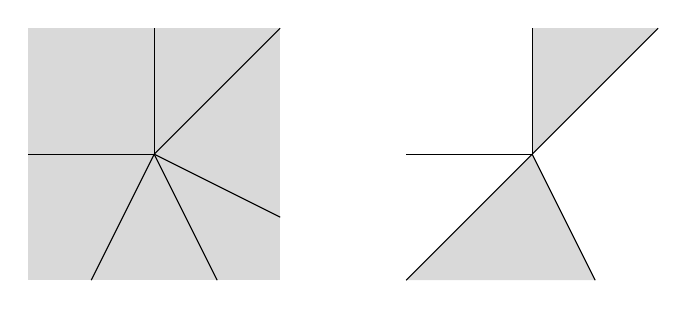
\begin{tikzpicture}[scale=1.6]
        \fill[gray!30] (-1,-1) -- (1,-1) -- (1,1) -- (-1,1) -- cycle;
        \draw (0,0) -- (-1,0);
        \draw (0,0) -- (-0.5,-1);
        \draw (0,0) -- (0.5,-1);
        \draw (0,0) -- (1,-0.5);
        \draw (0,0) -- (1,1);
        \draw (0,0) -- (0,1);

        \begin{scope}[xshift=3cm]
            \fill[gray!30] (0,0) -- (-1,-1) -- (0.5,-1) -- cycle;
            \fill[gray!30] (0,0) -- (1,1) -- (0,1) -- cycle;

            \draw (0,0) -- (-1,0);
            \draw (0,0) -- (-1,-1);
            \draw (0,0) -- (0.5,-1);
            \draw (0,0) -- (1,1);
            \draw (0,0) -- (0,1);
        \end{scope}
    \end{tikzpicture}
    \caption{Polyhedral fans.}
    \label{fig:Polyfan}
\end{figure}

\begin{figure}[h!]
    \centering
    
\begin{tikzpicture}[scale=1.6]
        \fill[gray!30] (-1,-1) -- (1,-1) -- (1,1) -- (-1,1) -- cycle;
        \draw (1,0) -- (-1,0);
        \draw (0,0) -- (0,1);
        
    \end{tikzpicture}
    \caption{Not a polyhedral fan.}
    \label{fig:Notpolyfan}
\end{figure}


\begin{definition}
    A \textit{polyhedral fan} is a collection of polyhedral cones satisfying two conditions:
    \begin{enumerate}[label = \textit{(\arabic*)}]
        \item Every face of a cone in the fan is in the fan;
        \item The intersection of any two cones in the fan is a face of each cone.
    \end{enumerate}
\end{definition}

See Figures \ref{fig:Polyfan} and \ref{fig:Notpolyfan} for an illustration of this definition.

\begin{definition} 
    A polyhedral cone $C$ is \textit{simplicial} if there exists some linearly independent set of vectors $\textbf{v}_1,\ldots,\mathbf{v}_r$ such that $C = \text{pos}(\mathbf{v}_1,\ldots,\mathbf{v}_r)$. Consequently, a polyhedral fan is \textit{simplicial} if every cone is \textit{simplicial}.
\end{definition}

Note the similarity in definitions between a polyhedral cone and a polyhedron as well as the similarity in definitions of a polyhedral fan and a polyhedral complex. This is because polyhedral cones are special cases of polyhedra, and polyhedral fans are special cases of polyhedral complexes.

These polyhedral structures form the geometric foundation for understanding tropical varieties, which are unions of polyhedra arranged in specific combinatorial patterns.

\subsection{Newton Polygons \& Regular Subdivisions}\label{section:Newtpoly}
In tropical geometry, the Newton polytope serves as a fundamental link between algebraic and combinatorial structures. Newton polytopes are geometric objects that encode the combinatorial structure of a polynomial, representing the exponents of its monomials as points in a polytope in $\RR^n$.

In this section, we being by defining Newton polytopes and illustrating them with some key examples. We then go on to introduce the notion of regular subdivisions, which reflect the structure of the tropicalisation of polynomials. We conclude with the definition and examples of extended Newton polytopes that play a crucial role in the algorithms for computing tropical varieties. 


\begin{definition}
    (\cite[Def. 2.3.4]{MS2015})Let $S = K[x_1^{\pm1},\ldots,x_n^{\pm1}]$ be the Laurent polynomial ring. Given the polynomial $f=\sum_{\mathbf{u}\in\ZZ^n}c_{\mathbf{u}}\mathbf{x}^\mathbf{u}\in S$, the \textit{Newton polytope} of $f$ is the polytope \[\text{Newt}(f) \; = \; \text{conv}(\mathbf{u} \; | \;c_{\mathbf{u}} \neq 0) \, \subseteq \, \RR^n.\]
    This is called a Newton polygon if it is two dimensional.
\end{definition}

\begin{example}
\label{ex:NewtPoly}
    Let $S=\CC[x^{\pm1},y^{\pm1}]$. Consider the polynomial
    
    \[\begin{aligned}
    f &= x^3y + 4x^2y^2 +7x^2(2y - 1) - 7xy^2 + x +2y.\\
      &= x^3y + 4x^2y^2 +14x^2y - 7x^2 - 7xy^2 + x +2y     
    \end{aligned}\]
    
    
    The Newton polygon of $f$ is the convex hull of the points $(1,0),$ $(0,1),$ $(1,2),$ $(2,0),$ $(2,1),$ $(2,2)$ and $(3,1)$, which is shown in Figure \ref{fig:Newtpolygonex}.
\end{example}

\begin{figure}[h]
\centering
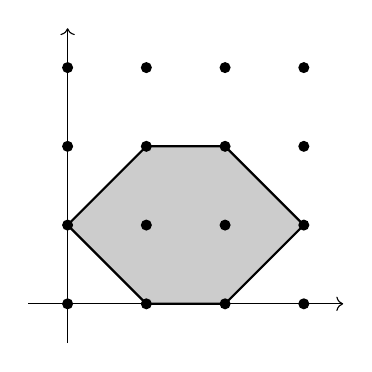
\begin{tikzpicture}[scale=1.0]

\draw[->] (-0.5,0) -- (3.5,0);
\draw[->] (0,-0.5) -- (0,3.5);

\fill[gray!40] (1,0) -- (2,0) -- (3,1) -- (2,2) -- (1,2) -- (0,1);
\draw[thick]   (1,0) -- (2,0) -- (3,1) -- (2,2) -- (1,2) -- (0,1) -- cycle;

\foreach \x in {0,1,2,3} {
    \foreach \y in {0,1,2,3} {
        \fill (\x,\y) circle (2pt);
    }
}

\end{tikzpicture}
\caption{The Newton polygon in Example \ref{ex:NewtPoly}.}
\label{fig:Newtpolygonex}
\end{figure}

A particular class of polyhedral complexes that we are interested in are \textit{regular subdivisions} of a polytope. A regular subdivision of a Newton polytope is a decomposition of the polytope into smaller convex polytopes, based on an assignment of weights to each point.

\begin{definition}
    Let $\mathbf{u}_1,\ldots,\mathbf{u}_r$ be a point configuration in $\RR^n$. The \textit{regular subdivision} of the polytope $P = \text{conv}\{\mathbf{u}_i \; |\; 1 \leq i \leq r\}$ induced by $\mathbf{w} = (w_1,\ldots,w_r) \in \RR^r$ has the following geometric description. We form the polytope 
    \[P_\mathbf{w} = \text{conv}\left\{ (\mathbf{u}_i,w_i) \; | \; 1 \leq i \leq r \right\} \subseteq \RR^{n+1}.\] The lower faces of $P_\mathbf{w}$ are those with an inner normal vector $\mathbf{c} \in (\RR^{n+1})^\vee$ with a positive last coordinate. These lower faces project down to $P \subseteq \RR^n$ and form a polyhedral complex whose support equals $P$. This is the \textit{regular subdivision} of $\mathbf{u}_1,\ldots,\mathbf{u}_r$ induced by the weight vector $\mathbf{w}$.
\end{definition}

By assigning weights to each point in the Newton polytope, we lift each point \(\mathbf{u}_i\) to \((\mathbf{u}_i, w_i) \in \mathbb{R}^{n+1}\), forming a new polytope in a higher dimension. We then compute the lower convex hull of these lifted points in $\RR^{n+1}$, meaning the faces of the polytope that are visible from below when viewed in the positive \(z\)-direction (i.e. whose inner normal has a positive last coordinate). Then we project the lower faces of the convex hull back to $\RR^n$, which results in the regular subdivision of the polytope.

\begin{definition}
    When each polytope in the polyhedral complex is a simplex, the subdivision is called a \textit{regular triangulation} of $P$.
\end{definition}

\begin{figure}[t]
\centering
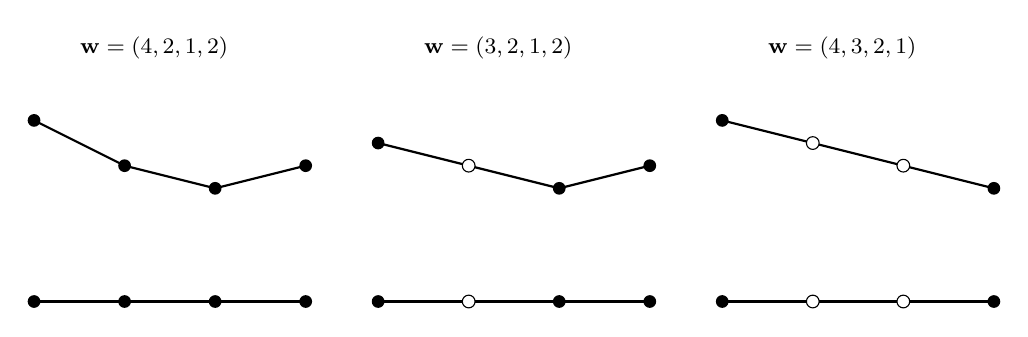
\begin{tikzpicture}[scale=1.15]

\draw[thick] (0,1) -- (1,0.5) -- (2, 0.25) -- (3,0.5);
\fill (0,1) circle (2pt);
\fill (1,0.5) circle (2pt);
\fill (2,0.25) circle (2pt);
\fill (3,0.5) circle (2pt);


\fill (0,-1) circle (2pt);
\fill (1,-1) circle (2pt);
\fill (2,-1) circle (2pt);
\fill (3,-1) circle (2pt);

\draw[thick] (0,-1) -- (3,-1);


\node[anchor = west] at (0.4,1.8) {\footnotesize $\mathbf{w} = (4,2,1,2)$};

\begin{scope}[xshift=3.8cm]

\draw[thick] (0,0.75) -- (1,0.5) -- (2, 0.25) -- (3,0.5);
\fill (0,0.75) circle (2pt);
\fill[fill=white, draw=black] (1,0.5) circle (2pt);
\fill (2,0.25) circle (2pt);
\fill (3,0.5) circle (2pt);

\draw[thick] (0,-1) -- (0.93,-1);
\draw[thick] (1.07,-1) -- (3,-1);

\fill (0,-1) circle (2pt);
\draw (1,-1) circle (2pt);
\fill (2,-1) circle (2pt);
\fill (3,-1) circle (2pt);

\node[anchor = west] at (0.4,1.8) {\footnotesize $\mathbf{w} = (3,2,1,2)$};
\end{scope}

\begin{scope}[xshift=7.6cm]
\draw[thick] (0,1) -- (1,0.75) -- (2, 0.50) -- (3,0.25);
\fill (0,1) circle (2pt);
\fill[fill=white, draw=black] (1,0.75) circle (2pt);
\fill[fill=white, draw=black] (2,0.5) circle (2pt);
\fill (3,0.25) circle (2pt);


\draw[thick] (0,-1) -- (0.93,-1);
\draw[thick] (1.07,-1) -- (1.93,-1);
\draw[thick] (2.07,-1) -- (3,-1);

\fill (0,-1) circle (2pt);
\draw (1,-1) circle (2pt);
\draw (2,-1) circle (2pt);
\fill (3,-1) circle (2pt);

\node[anchor = west] at (0.4,1.8) {\footnotesize $\mathbf{w} = (4,3,2,1)$};

\end{scope}

\end{tikzpicture}
\caption{Some examples of regular subdivisions.}
\label{fig:regularsubs}
\end{figure} % 1-dimensional example


\begin{example}
    Let's look at some examples to help illustrate what regular subdivisions look like.
    \begin{enumerate}
        \item[(1)] Let $n =1$, $r = 4$. Consider the points $0,1,2,3$ on the line $\RR^1 = \RR$. The convex hull of the points is simply the line segment $[0,3]$. If $\mathbf{w} = (4,2,1,2)$, then the regular triangulation consists of the three line segments: $[0,1], [1,2] $ and $[2,3]$. For the weight vector $\mathbf{w} = (3,2,1,2)$ there are two line segments: $[0,2]$ and $[2,3]$. For $\mathbf{w}=(4,3,2,1)$ there is only one line segment: $[0,3]$. The convex hulls of the points can be seen at the top of Figure \ref{fig:regularsubs} as well as the regular subdivisions at the bottom of the figure.

        \item[(2)] Let $n = 2$ and $r = 6$. Fix the points $(2,0)$, $(1,1)$, $(0,2)$, $(1,0)$, $(0,1)$ and $(0,0) \in \RR^2$. Let $\mathbf{w} = (1,0,1,0,0,2)$, so we assign these weights to each point we lift the polytope into $\RR^3$. We then take the lower faces of the convex hull of these lifted coordinates and project it back to $\RR^2$. This results in a triangulation with four triangles. The process to compute the regular triangulation can be seen in Figure \ref{fig:triangulationprocess}. For $\mathbf{w} = (3,0,3,1,1,0)$ the triangulation has four triangles again, but they are arranged differently from the first one due to the different points being lifted. Finally, for $\mathbf{w} = (0,0,0,0,0,0)$ the triangulation is just the one triangle of the outer points as no points have been lifted. The regular triangulations induced by the three weight vectors in this example can be seen in Figure \ref{fig:regtriangualation}.
    \end{enumerate}
\end{example}





\begin{figure}
\centering
\tdplotsetmaincoords{120}{70} % Set viewing angle: (elevation, azimuth)
\begin{tikzpicture}


\begin{scope}[tdplot_main_coords]

\draw[thick,->] (-1,0,0) -- (3.5,0,0) node[anchor=south west]{$y$};
\draw[thick,->] (0,-1,0) -- (0,2.7,0) node[anchor=north west]{$x$};
\draw[thick,->] (0,0,-1) -- (0,0,3) node[anchor=south]{$z$};

\draw[thick] (1,0,0) -- (0,1,0) -- (1,1,0) -- cycle;
\fill[blue!20] (1,0,0) -- (0,1,0) -- (1,1,0) -- cycle;

\draw[thick] (1,1,0) -- (0,1,0) -- (0,2,1) -- cycle;
\fill[red!20] (1,1,0) -- (0,1,0) -- (0,2,1) -- cycle;

\draw[thick] (1,1,0) -- (1,0,0) -- (2,0,1) -- cycle;
\fill[green!20] (1,1,0) -- (1,0,0) -- (2,0,1) -- cycle;

\fill (1,0,0) circle (2pt);

\draw[thick] (0,1,0) -- (1,0,0) -- (0,0,2) -- cycle;
\fill[yellow!20] (0,1,0) -- (1,0,0) -- (0,0,2) -- cycle;

\fill (0,0,2) circle (2pt);
\fill (0,1,0) circle (2pt);
\fill (1,1,0) circle (2pt);
\fill (2,0,1) circle (2pt);
\fill (0,2,1) circle (2pt);

\end{scope}

\begin{scope}[xshift = 3.5cm]
    \node[anchor = west] at (0.65,1.2) {$\RR^3 \to \RR^2$};
    \draw[->, very thick] (-0.2,0.9) -- (3.2,0.9);
    \node[anchor = west] at (0,0.6) {$(x,y,z) \mapsto (x,y)$};

     
\end{scope}

\begin{scope}[xshift = 7.7cm, yshift = -0.4cm]
    \draw[thick,->] (-0.5,0) -- (2.9,0) node[anchor=north]{$x$};
    \draw[thick,->] (0,-0.5) -- (0,2.9) node[anchor=south]{$y$};
    
    \draw[thick] (1,0) -- (0,1) -- (1,1) -- cycle;
    \fill[blue!20] (1,0) -- (0,1) -- (1,1) -- cycle;
    
    \draw[thick] (1,1) -- (0,1) -- (0,2) -- cycle;
    \fill[green!20] (1,1) -- (0,1) -- (0,2) -- cycle;
    
    \draw[thick] (1,1) -- (1,0) -- (2,0) -- cycle;
    \fill[red!20] (1,1) -- (1,0) -- (2,0) -- cycle;
    
    \draw[thick] (0,1) -- (1,0) -- (0,0) -- cycle;
    \fill[yellow!20] (0,1) -- (1,0) -- (0,0) -- cycle;

    \fill (0,0) circle (2pt);
    \fill (1,0) circle (2pt);
    \fill (0,1) circle (2pt);
    \fill (1,1) circle (2pt);
    \fill (2,0) circle (2pt);
    \fill (0,2) circle (2pt);
\end{scope}
\end{tikzpicture}
\caption{Constructing a regular triangulation.}
\label{fig:triangulationprocess}
\end{figure} % Construction


\begin{figure}[b]
    \centering
    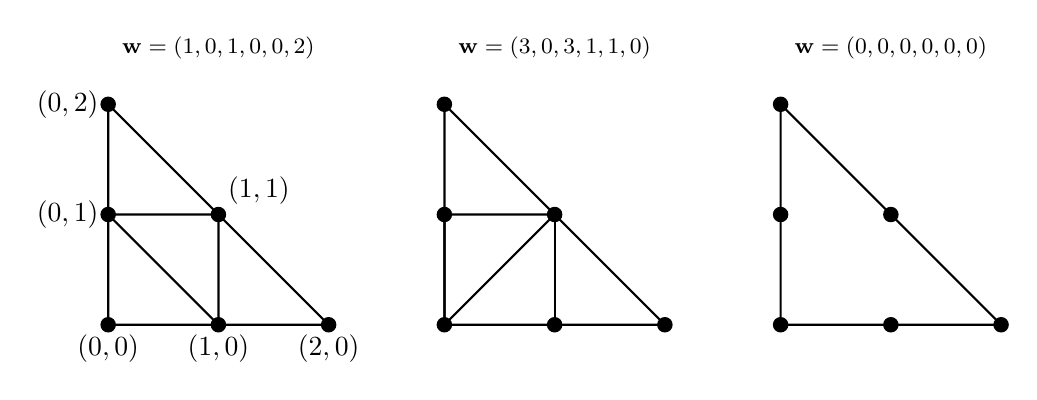
\begin{tikzpicture}[scale = 1.4]       
    
    \begin{scope}
    
    \draw[thick] (0,0) -- (1,0) -- (2,0) -- (1,1) -- (0,2) -- (0,1) -- cycle;
    \draw[thick] (1,0) -- (0,1) -- (1,1) -- cycle;   

    \fill (0,0) circle (2pt) node[anchor=north]{$(0,0)$};
    \fill (1,0) circle (2pt) node[anchor=north]{$(1,0)$};
    \fill (0,1) circle (2pt) node[anchor=east]{$(0,1)$};
    \fill (1,1) circle (2pt) node[anchor=south west]{$(1,1)$};
    \fill (2,0) circle (2pt) node[anchor=north]{$(2,0)$};
    \fill (0,2) circle (2pt) node[anchor=east]{$(0,2)$};

    \node[anchor = north] at (1,2.7) {\footnotesize $\mathbf{w} = (1,0,1,0,0,2)$};

    
    \end{scope}

    \begin{scope}[xshift = 3.05cm]

    \draw[thick] (0,0) -- (1,0) -- (2,0) -- (1,1) -- (0,2) -- (0,1) -- cycle;
    \draw[thick] (0,0) -- (0,1) -- (1,1) -- cycle;   
    \draw[thick] (1,0) -- (1,1);   

    \foreach \x/\y in {0/0, 1/0, 2/0, 0/1, 1/1, 0/2}
    \fill[black] (\x,\y) circle (2pt);

    \node[anchor = north] at (1,2.7) {\footnotesize $\mathbf{w} = (3,0,3,1,1,0)$};

    \end{scope}

    \begin{scope}[xshift = 6.1cm]
      
    \draw[thick] (0,0) -- (1,0) -- (2,0) -- (1,1) -- (0,2) -- (0,1) -- cycle;

    \foreach \x/\y in {0/0, 1/0, 2/0, 0/1, 1/1, 0/2}
    \fill[black] (\x,\y) circle (2pt);

    \node[anchor = north] at (1,2.7) {\footnotesize $\mathbf{w} = (0,0,0,0,0,0)$};

    \end{scope}
    
    \end{tikzpicture}
    \caption{Some examples of regular triangulations.}
    \label{fig:regtriangualation}
\end{figure} % Regular triangulations

The following definition will be crucial for the understanding of the algorithms for computing tropical varieties, which we will present in subsequent sections.

\begin{definition}
    (\cite[Def. 2.6]{HR2018}) For a univariate polynomial $f=\sum_{i=0}^dc_i\cdot x_k^i \in K[x_k]$, $c_i \in K$, the \textit{extended Newton polyhedron} is defined to be \[\Delta(f) := \text{conv}\bigl(\{ (i,\val(c_i)) \; | \;  c_i \neq 0  \}\bigr) + (\{0\} \times \RR_{\geq0}).\] Similarly, for a multivariate polynomial $f=\sum_{i=0}^df_i\cdot x_k^i \in K[x_1,\ldots,x_k]$, $f_i \in K[x_1,\ldots,x_{k-1}]$, and a weight $w \in \RR^{k-1}$, we define the \textit{expected Newton polygon} of $f$ at $w$ to be \[\Delta_w(f):= \text{conv}\bigl( \{ (i, \trop(f_i)(w)) \; | \; f_i \neq 0 \}\bigr) + (\{0\} \times \RR_{\geq0}).\]
\end{definition}

\begin{remark}
    For the rest of this report, we will use the term Newton polygon to describe the extended Newton polyhedron as defined above, for $n = 1$.
\end{remark}

\begin{example}
    We present two examples to show the extended Newton polygon of a univariate polynomial and the expected Newton polygon for a multivariate polynomials. 
    \begin{enumerate}
        \item[(1)] Consider the univariate polynomial $g = tx^2 + x + 5 \in \puiseux$. We need to compute the valuation of the coefficients in each term. Here we have $\val(c_2 = t) = 1$, $\val(c_1 = 1) = 0$ and $\val(c_0 = 5) = 0$. So the Newton polygon of $g$ is \[\Delta(g) = \text{conv}((0,0), (1,0)) + (\{0\} \times \RR_{\geq0}).\] This is shown on the left of Figure \ref{fig:extendedNewton}.
        \item[(2)] Let's look at a multivariate example. Consider the polynomial \\$ g = 2x_0^3 + x_0x_2 + x_0 + 3x_1x_2^2 + x_2 + 4 \in \QQ_2[x_0,x_1,x_2]$ and fix $w = (1,2)$. So here we have the polynomials \[g_0 = 2x_0^3 + x_0 + 4, \quad g_1 = x_0 + 1, \quad g_2 = 3x_1,\] where $g_i \in \QQ_2[x_0,x_1]$. We then need to compute $\trop(g_i)(w)$. The tropicalisation of $g_0$ is $\trop(g_0)(w) = \min(2+3(1), 1, 2) = 1.$ Similarly $\trop(g_1)(w) = 0$ and $\trop(g_2)(w) = 2$. So the Newton polygon of $g$ at $w$ is \[\Delta_w(g) = \text{conv}((0,1), (1,0), (2,2)) + (\{0\} \times \RR_{\geq0})\] and is shown on the right of Figure \ref{fig:extendedNewton}. 
    \end{enumerate}
\end{example}

\begin{figure}
    \centering
    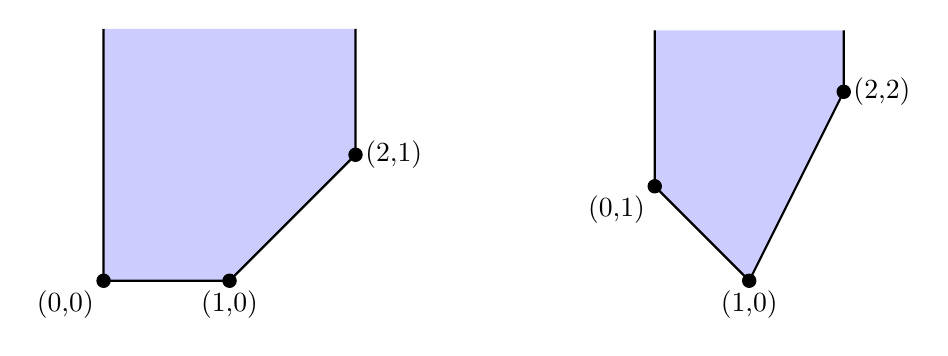
\begin{tikzpicture}
        \begin{scope}[scale = 1.6]
        
        \fill[blue!20] (0,2) -- (0,0) -- (1,0) -- (2,1) -- (2,2);
        \draw[thick] (0,2) -- (0,0) -- (1,0) -- (2,1) -- (2,2);
        
        \filldraw[black] (0,0) circle (1.5pt) node[anchor=north east] {(0,0)};
        \filldraw[black] (1,0) circle (1.5pt) node[anchor=north] {(1,0)};
        \filldraw[black] (2,1) circle (1.5pt) node[anchor=west] {(2,1)};
        
        \end{scope}
        
        \begin{scope}[xshift = 7cm, scale = 1.2]
        
        \fill[blue!20] (0,2.65) -- (0,1) -- (1,0) -- (2,2) -- (2,2.65);
        \draw[thick] (0,2.65) -- (0,1) -- (1,0) -- (2,2) -- (2,2.65);
        
        \filldraw[black] (0,1) circle (2pt) node[anchor=north east] {(0,1)};
        \filldraw[black] (1,0) circle (2pt) node[anchor=north] {(1,0)};
        \filldraw[black] (2,2) circle (2pt) node[anchor=west] {(2,2)};
        
        \end{scope}


    \end{tikzpicture}
    \caption{Examples of extended and expected Newton polygons.}
    \label{fig:extendedNewton}
\end{figure}


\subsection{Initials \& Stars}
\label{sec:initials}
In tropical geometry, the concept of an initial form plays a crucial role in understanding tropical varieties. Given a polynomial with coefficients in a valued field, the initial form extracts the dominant terms with respect to a weight vector. This section introduces the initial form, provides formal definitions, and illustrates its computation with examples. Later in the section, we introduce the define and give examples of stars of cells in a polyhedral complex. The star describes the local structure around a face and is a fundamental building block in the local study of tropical varieties.

\begin{definition}
    Let's start with the polynomial \[f \; = \sum_{\mathbf{u}\in\NN^n}c_\mathbf{u}x^\mathbf{u} \in K[x_1,\ldots,x_n].\] Fix a \textit{weight vector} $\mathbf{w} = (w_1,\ldots,w_n)\in\Gamma_{\val}^{n}$, and let \[W = \trop(f)(\mathbf{w}) = \min\{ \val(c_{\mathbf{u}}) + \mathbf{w} \cdot \mathbf{u} \;|\; c_{\mathbf{u}}\neq 0\}.\] Then the \textit{initial form} of $f$ with respect to $\mathbf{w}$ is
    \begin{equation*}
        \initial_{\mathbf{w}}(f) \; = \; \sum_{\substack{\mathbf{u}\in\NN^{n}: \\ \val(c_\mathbf{u}) + \mathbf{w}\cdot\mathbf{u} = W}} \overline{c_{\mathbf{u}}p^{-\val(c_\mathbf{u})}x^{\mathbf{u}}}\;.
    \end{equation*}

    Alternatively, when $\mathbf{w}\in\Gamma_{\val}^{n}$, the initial form can be expressed in terms of a rescaling transformation 
    \begin{equation*}
        \initial_{\mathbf{w}}(f) \; = \; \overline{p^{-W} \sum_{\mathbf{u}\in\NN^{n}}c_{\mathbf{u}}p^{\mathbf{w}\cdot\mathbf{u}}x^{\mathbf{u}} } \; = \; \overline{p^{-\trop(f)(\mathbf{w})}f(p^{w_1}x_1,\ldots,p^{w_n}x_n)}\;.
    \end{equation*}
\end{definition}

The initial form of a polynomial $\initial_{\mathbf{w}}(f)$ extracts the dominant terms relative to a weight vector $\mathbf{w}$. The definition relies on using the valuation to evaluate the monomials in the tropical polynomial and selecting the monomials that achieve the minimum valuation. Taking the reduction modulo the valuation ensures that only the dominant terms remain, essentially removing all positive powers of $p$.

\begin{example}
    Consider the polynomial \[f = t^2x_0 + (t+t^3)x_1 + 2t^2x_2x_3 \in \puiseux[x_0,x_1,x_2,x_3].\]
    Let $\mathbf{w} = (0,0,0,0)$. Then we compute:
    \begin{align*}
        \val(t^2) &= 2, \\
        \val(t+t^3&) = 1, \\
        \val(2t^2) &= 2.
    \end{align*}
    So $\trop(f)(\mathbf{w}) = \min(2,1,2) = 1$, and the initial form is \[\initial_{\mathbf{w}}(f) = \overline{(1 + t^2)x_1} = x_1.\]
    Now let $\mathbf{w} = (2,4,1,1)$. We compute:
    \begin{align*}
        \val(t^2) + \mathbf{w}\cdot(1,0,0,0) = 2 + 2 = 4&, \\
        \val(t+t^3) + \mathbf{w}\cdot(0,1,0,0) = 1 + 4 =& \; 5, \\
        \val(2t^2) + \mathbf{w}\cdot(0,0,1,1) = 2 + (1+1) &= 4.
    \end{align*}

    
    Then $\trop(f)(\mathbf{w}) = \min(4,5,4) = 4$, and
    \[\initial_{\mathbf{w}}(f) = x_0 + 2x_2x_3.\]
\end{example}

\begin{definition}
    The initial ideal of ideal $I$ with respect to $\mathbf{w}$ is $\initial_{\mathbf{w}}(I) = \langle\initial_{\mathbf{w}}(f) \; | \; f \in I \rangle.$
\end{definition}

The initial ideal captures the leading (lowest weight) terms of all the generators of the ideal $I$ and plays a central role in Gröbner theory,
both classical and tropical.

\begin{definition}
    (\cite[Def. 2.3.6]{MS2015}) Let $\Sigma$ be a polyhedral complex in $\RR^n$ and let $\sigma$ be a cell in $\Sigma$. The \textit{star} of $\sigma$ in $\Sigma$ is a fan in $\RR^n$, denoted by $\text{star}_{\Sigma}(\sigma)$. Its cones are indexed by those cells $\tau$ in $\Sigma$ that contain $\sigma$ as a face. The cone of $\text{star}_{\Sigma}(\sigma)$ that is indexed by $\tau$ is the following subset of $\RR^n$: \[\overline{\tau} = \{\lambda(\mathbf{u} - \mathbf{v}) \; | \; \lambda\geq 0, \mathbf{u}\in\tau,\mathbf{v}\in\sigma \}\]
\end{definition}

The star captures the local structure of the complex near the cell $\sigma$ and is a key ingredient in the definition of tropical varieties via local fans.

\begin{example}
    The polyhedral complex shown on the left of Figure \ref{fig:starex} is a quadratic curve in the tropical plane. The affine span of the vertex $\sigma_1$ in the polyhedral complex $\Sigma$ is just the vertex itself. The star is shown on the top right of the figure. For $\sigma_2$ the affine span is the entire y-axis, which is also the star.
\end{example}

\begin{figure}[h]
    \centering
    \begin{tikzpicture}[scale = 1.2]
        \begin{scope}
            \draw[thick] (0,0) -- (1,1) -- (2,1);
            \draw[thick] (1,1) -- (1,2);
            \draw[thick] (0,0) -- (0,-1) -- (2,-1);
            \draw[thick] (0,-1) -- (-1,-2);
            \draw[thick] (0,0) -- (-1,0) -- (-2,-1);
            \draw[thick] (-1,0) -- (-1,2);

            \draw[-{Latex[length=2mm]}] (1.4,1.4) -- (1.1,1.1);
            \node at (1.6,1.5) {\small$\sigma_1$};

            \draw[-{Latex[length=2mm]}] (0.4,-.5) -- (0.05,-0.5);
            \node at (0.6,-0.5) {\small$\sigma_2$};
        \end{scope}

        \begin{scope}[xshift = 5cm] 
            \draw[thick] (0,0) -- (1,1) -- (2,1);
            \draw[thick] (1,1) -- (1,2);

            \node[anchor = west] at (1.2,2.2) {$\text{star}_\Sigma(\sigma_1)$};

        \end{scope}

        \begin{scope}[xshift = 5cm, yshift=-1cm]
            \draw[thick] (1,-1) -- (1,1);
            \node[anchor = west] at (1.2,0) {$\text{star}_\Sigma(\sigma_2)$};
        \end{scope}        
    \end{tikzpicture}
    \caption{The star of a polyhedron in a polyhedral complex.}
    \label{fig:starex}
\end{figure}

\section{Tropical Varieties}
In this section, we introduce the notion of tropical varieties. To build a general understanding of tropical varieties, we begin by introducing a simple and fundamental case: tropical hypersurfaces. These are tropicalisations of single polynomials and offer a great entry point before we then extend the discussion to the tropicalisation of more general algebraic varieties. We will use some of the key concepts in tropical geometry that we introduced in Section \ref{sec:2} to both define tropical varieties and study their relations with tropical varieties.

\begin{contribution*}
    Throughout this section, we present definitions, theorems, and some examples that are taken from Chapters 3.1 and 3.2 of \cite{MS2015}. All the figures appearing in this section are produced by me and where applicable, I have provided my own explanations to further help the understanding and provide context for the later sections of this report.
\end{contribution*}

\subsection{Tropical Hypersurfaces}
% Change R^3 to an algebraically closed field 
A hypersurface is a special case of a variety which is defined by a single polynomial equation. They are codimension-one varieties, which means that the dimension of the variety is one less than the dimension of the ambient space that the hypersurface is in. For example, in $\CC^3$, a surface like a plane or a sphere is a two-dimensional hypersurface and in $\CC^2$, a curve is a one-dimensional hypersurface.


Let K be an arbitrary valued field. We consider the ring $K[x_1^{\pm1},\ldots,x_n^{\pm1}]$ of Laurent polynomials over $K$. For a Laurent polynomial $f = \sum_{\mathbf{u}\in\ZZ^n}c_\mathbf{u}x^\mathbf{u}$, we define its tropicalisation $\displaystyle \trop(f) = \min_{\mathbf{u}\in \ZZ^n}\left( \val(c_\mathbf{u}) + \mathbf{u}\cdot\mathbf{w} \right)$ as in (\ref{eqn:tropicalpoly}).

The classical variety of the Laurent polynomial $f \in K[x_1^{\pm1},\ldots,x_n^{\pm1}]$ is a hypersurface in the algebraic torus $(K^*)^n$ over the algebraic closure of $K$: 
\[V(f) \; = \; \{\mathbf{y}\in T^n \; | \; f(\mathbf{y}) = 0 \}.\]

We now go on to define the tropical hypersurface for $f$.

\begin{definition}
    (\cite[Def. 3.1.1]{MS2015}) The \textit{tropical hypersurface} $\trop(V(f))$ is the set \[\{\mathbf{w} \in \RR^n \; | \; \text{the minimum in } \trop(f)(\mathbf{w)} \text{ is achieved at least twice}\}.\]

    This is the locus in $\RR^n$ where the piecewise linear function $\trop(f)$ fails to be linear. 
    
    Alternatively, this can also be defined in terms of initial forms as introduced in Section \ref{sec:initials}. The tropical hypersurface $\trop(V(f))$ is the set of weight vectors $\mathbf{w}\in \RR^n$ for which the initial form $\initial_\mathbf{w}(f)$ is not a monomial. 
\end{definition}


\begin{figure}
    \centering
    \begin{tikzpicture}
        \begin{scope}[scale = 1.5]
            \draw[thick] (0,0) -- (2,0);
            \draw[thick] (0,0) -- (0,2);
            \draw[thick] (0,0) -- (-2,-2);
            \node[anchor = south west] at (0,0) {$(0,0)$};

            
        \end{scope}

        \begin{scope}[xshift = 6.3cm, scale = 0.55] 
            \node[anchor = west] at (-0.9,-0.2) {$(-1,0)$};

            \node[anchor = south east] at (-2.1,-0.2) {$(-2,0)$};
            \draw[thick] (-1,0) -- (-2,0);
                \draw[thick] (-4,-2) -- (-2,0);
                \draw[thick] (-2,6) -- (-2,0);
            \node[anchor = south west] at (-0.9,-3) {$(-1,-3)$};
            \draw[thick] (-1,0) -- (-1,-3);
                \draw[thick] (-3,-5) -- (-1,-3);
                \draw[thick] (5,-3) -- (-1,-3);
            \node[anchor = north west] at (2.9,4) {$(3,4)$};      
            \draw[thick] (-1,0) -- (3,4);
                \draw[thick] (3,6) -- (3,4);
                \draw[thick] (5,4) -- (3,4);            
        \end{scope}     
    \end{tikzpicture}
    \caption{A tropical line and a tropical quadric.}
    \label{fig:tropicallinequadric}
\end{figure}

\begin{example}
    (\cite[Ex. 3.1.2]{MS2015}) Let $K = \puiseux$ and we consider bivariate polynomials $f\in K[x^{\pm1},y^{\pm1}].$
    \begin{enumerate}[left = 1.9em]
        \item[(1)] Let $f=x+y+1.$ Then $\trop(f)(\mathbf{w}) = \min(w_1,w_2,0)$, so \\$\trop(V(f))(\mathbf{w}) = \{w_1 = w_2 \leq 0\} \cup \{w_1=0 \leq w_2\} \cup \{ w_2=0 \leq w_1\}.$ This tropical line is shown on the left in Figure \ref{fig:tropicallinequadric}.
        \item[(2)] Consider the polynomial \[f=t^2x^2 + xy + (t^2+t^3)y^2 + (1+t^3)x + t^{-1}y + t^3.\] Then we have \[\trop(f)(\mathbf{w}) = \min(2+2w_1, w_1+w_2, 2+2w_2, w_1, -1+w_2, 3),\] so $\trop(V(f))$ consists of the three line segments that join the pairs $\{(-1,0),(-2,0)\}$, $\{(-1,0),(-1,-3)\}$, $\{(-1,0),(3,4)\}$, and the six rays $\{(-2,0) + \lambda(0,1)\}$, $\{(-2,0) - \lambda(1,1)\}$, $\{(-1,-3) - \lambda(1,1)\}$, $\{(-1,-3) + \lambda(1,0)\}$, $\{(3,4) + \lambda(0,1)\}$, $\{(3,4) + \lambda(1,0)\}$, where in these sets, $\lambda$ runs over $\RR_{\geq0}$. This is shown on the right of Figure \ref{fig:tropicallinequadric}.
    \end{enumerate}
\end{example}

The following theorem establishes a link between hypersurfaces in classical algebra over a field $K$ and tropical hypersurfaces in $\RR^n$. The proof of this theorem can be found in Chapter 3.1 of \cite{MS2015}.

\begin{theorem}[Kapranov Theorem] \label{Thm:Kapranov}
    (\cite[Thm. 3.1.3]{MS2015}) Let $K$ be an algebraically closed field with a nontrivial valuation $\val$. Fix a Laurent polynomial $f = \sum_{\mathbf{u}\in\ZZ^n}c_{\mathbf{u}}x^{\mathbf{u}}$ in the polynomial ring $K[x_1^{\pm1},\ldots,x_n^{\pm1}].$ The following three sets coincide:
    \begin{enumerate}
        \item[(1)] the tropical hypersurface $\trop(V(f))$ in $\RR^n$;
        \item[(2)] the set $\{\mathbf{w}\in\RR^n\; | \; \initial_{\mathbf{w}}(f) \text{ is not a monomial }\}$;
        \item[(3)] the closure in $\RR^n$ of $\{(\val(y_1),\ldots,\val(y_n)) \; | \; (y_1,\ldots,y_n)\in V(f) \}$.
    \end{enumerate}
    
\end{theorem}

We will now consider an example to verify the equivalence between the three sets in Kopranov's theorem.

\begin{example}
    Consider the polynomial $f = x - y +1 \in K[x^{\pm1},y^{\pm1}]$, where $K$ is an algebraically closed field with a nontrivial valuation. Then we have the algebraic variety $V(f) = \{(z,z+1) \; | \; z\in K, z \neq 0 , -1\}$ and $\trop(V(f))$ is the tropical line shown in Figure \ref{fig:tropicallinequadric}.
    Now let us evaluate the second set in Kapranov's Theorem. Note that $\initial_\mathbf{w}(f)$ is a monomial unless either $\mathbf{w}$ is $(0,0)$, or $\mathbf{w}$ is a positive multiple of $(1,0), (0,1)$ or $(-1,-1)$. In these cases we have
    \[\initial_\mathbf{w}(f) = 
    \begin{cases}
        x-y+1 & \mathbf{w} = (0,0) \\
        -y+1 & \mathbf{w} = \alpha(1,0) \\
        x+1 & \mathbf{w} = \beta(0,1) \\
        x-y & \mathbf{w} = \gamma(-1,-1),
    \end{cases}\] where  $\alpha, \beta, \gamma \in \RR_{\geq0}$. The set of $\mathbf{w}$ where $\initial_\mathbf{w}(f)$ is not a monomial describes the tropical line in Figure \ref{fig:tropicallinequadric}. For the final set, where we take the closure of the set of coordinatewise valuations of points in $V(f)$, we have
    \[
        \left( \val(z), \val(z+1) \right) =
        \begin{cases}
        (\val(z), 0) & \text{if } \val(z) > 0, \\
        (\val(z), \val(z)) & \text{if } \val(z) < 0, \\
        (0, \val(z+1)) & \text{if } \val(z) = 0, \val(z+1) > 0, \\
        (0, 0) & \text{otherwise}.
        \end{cases} \]
    As $z$ runs over $K\setminus\{0,-1\}$, the above cases describe all the points of $\Gamma_{\val}^2$ that lie in the tropical line $\trop(V(f))$. As $K$ is algebraically closed, the value group $\Gamma_{\val}$ is dense in $\RR$, and so the closure of these points in $\Gamma_{\val}^2$ is the entire tropical line in $\RR^2$. So we can see that this confirms Theorem \ref{Thm:Kapranov} for this $f$.
\end{example}

Before we move on to study more general tropical varieties, I want to highlight the combinatorics of tropical hypersurfaces. We will use the idea of regular subdivisions from Section \ref{section:Newtpoly}.

The tropical hypersurface $\trop(V(f))$ is combinatorially dual to the regular subdivision of the Newton polygon of $f = \sum c_\textbf{u}x^{\textbf{u}}$ induced by the weights $\val(c_\textbf{u})$. Each cell in the tropical hypersurface corresponds to a face in the regular subdivison of complementary dimension. We say that $\trop(V(f))$ is the $(n-1)$-skeleton of the polyhedral complex dual to the regular subdivision. By the $(n-1)$-skeleton of a polyhedral complex $\Sigma$, we mean the polyhedral complex consisting of all cells $\sigma \in \Sigma$ such that $\text{dim}(\sigma) \leq n-1$. The explicit proof of this can be found in Chapter 3.1 of \cite{MS2015}.

We will now look at examples to highlight the duality between tropical hypersurfaces and said regular subdivisions.

\begin{figure}[t]
    \centering
    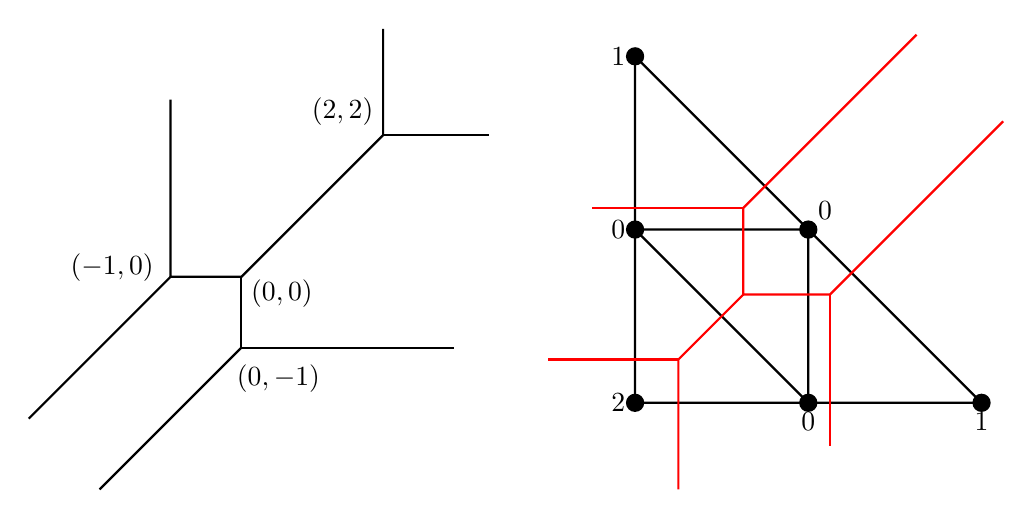
\begin{tikzpicture}
    \begin{scope}[scale = 0.9]
        \draw[thick] (-1,2.5) -- (-1,0) -- (0,0) -- (2,2) -- (2,3.5);
        \draw[thick] (-3,-2) -- (-1,0);
        \draw[thick] (2,2) -- (3.5,2);
        \draw[thick] (0,0) -- (0,-1) -- (3,-1);
        \draw[thick] (0,-1) -- (-2,-3);

        \node[anchor = south east] at (-1.1,-0.2) {$(-1,0)$};
        \node[anchor = north west] at (0,0.1) {$(0,0)$};
        \node[anchor = north west] at (-0.2,-1.1) {$(0,-1)$};
        \node[anchor = south east] at (2,2) {$(2,2)$};

    \end{scope}
    \begin{scope}[xshift = 5cm, yshift = -1.6cm, scale = 1.1]
        \fill (0,0) circle (3pt) node[anchor = east]{$2$};
    

        \fill (2,0) circle (3pt) node[anchor = north]{$0$};
        \fill (0,2) circle (3pt) node[anchor = east]{$0$};
        \fill (2,2) circle (3pt) node[anchor = south west]{$0$}; 
        \fill (4,0) circle (3pt) node[anchor = north]{$1$};
        \fill (0,4) circle (3pt) node[anchor = east]{$1$};
        \draw[thick] (0,0) -- (2,0) -- (4,0) -- (2,2) -- (0,4) -- (0,2) -- cycle;
        \draw[thick] (2,0) -- (0,2) -- (2,2) -- cycle; 
    
        

        \draw[thick, red] (3.25,4.25) -- (1.25,2.25) -- (1.25,1.25) -- (2.25,1.25) -- (4.25, 3.25);
        \draw[thick, red] (1.25,2.25) -- (-0.5, 2.25);
        \draw[thick, red] (2.25,1.25) -- (2.25,-0.5);
        \draw[thick, red] (1.25,1.25) -- (0.5,0.5) -- (0.5, -1);
        \draw[thick, red] (0.5,0.5) -- (-1, 0.5);
        \end{scope}

    \end{tikzpicture}
    \caption{A tropical curve and a visual aid for the duality.}
    \label{fig:dualityconstruction}
\end{figure}

\begin{figure}
    \centering
    \begin{tikzpicture}[scale = 0.8]
    \begin{scope}
        \draw[thick] (-4,-1) -- (-2,1) -- (-1,1) -- (1,-1) -- (1,-2) -- (-1,-4);
        \draw[thick] (-2,1) -- (-2,3);
        \draw[thick] (-1,1) -- (-1,3);
        \draw[thick] (1,-1) -- (3,-1);
        \draw[thick] (1,-2) -- (3,-2);
        
        \node[anchor = south east] at (-2,0.9) {$(-2,1)$};
        \node[anchor = south west] at (-1,1) {$(-1,1)$};
        \node[anchor = south west] at (0.9,-1) {$(1,-1)$};
        \node[anchor = north west] at (0.9,-2) {$(1,-2)$};

    \end{scope}
    \begin{scope}[xshift = 7.5cm, yshift = -0.7cm, scale = 1.2]
        \draw[thick] (-2,-2) -- (0,0) -- (3,0);
        \draw[thick] (0,0) -- (0,3);
        
        \node[anchor = south west] at (0,0) {$(0,0)$};
        
    \end{scope}

    \end{tikzpicture}
    \caption{Tropical curves from Example \ref{ex:duality}.}
    \label{fig:dualityexamples}
\end{figure}


\begin{figure}
    \centering
    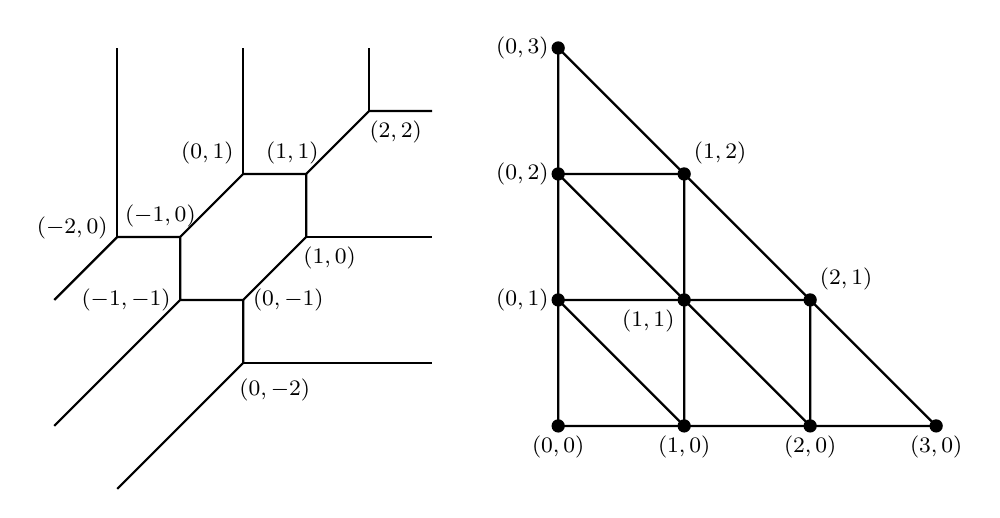
\begin{tikzpicture}[scale = 0.8, font = \footnotesize]
    \begin{scope}
        \draw[thick] (-3,-3) -- (-1,-1) -- (-1,0) -- (0,1) -- (1,1) -- (1,0) -- (0,-1) -- (-1,-1);
        \draw[thick] (1,1) -- (2,2) -- (3,2);
        \draw[thick] (2,2) -- (2,3);
        \draw[thick] (0,1) -- (0,3);
        \draw[thick] (1,0) -- (3,0);
        \draw[thick] (-1,0) -- (-2,0) -- (-3,-1);
        \draw[thick] (-2,0) -- (-2,3);
        \draw[thick] (0,-1) -- (0,-2) -- (-2,-4);
        \draw[thick] (0,-2) -- (3,-2);

        \node[anchor = east] at (-1,-1) {$(-1,-1)$};
        \node[anchor = south east] at (-0.6,0) {$(-1,0)$};
        \node[anchor = south east] at (0,1) {$(0,1)$};
        \node[anchor = south east] at (1.35,1) {$(1,1)$};
        \node[anchor = north west] at (0.8,0) {$(1,0)$};
        \node[anchor = west] at (0,-1) {$(0,-1)$};
        \node[anchor = north] at (0.5,-2.1) {$(0,-2)$};
        \node[anchor = east] at (-2,0.15) {$(-2,0)$};
        \node[anchor = north west] at (1.85,2) {$(2,2)$};

    \end{scope}

    \begin{scope}[xshift = 5cm, yshift = -3cm]
        \fill (0,0) circle (3pt) node[anchor=north]{$(0,0)$};
        \fill (2,0) circle (3pt) node[anchor=north]{$(1,0)$};
        \fill (0,2) circle (3pt) node[anchor=east]{$(0,1)$};
        \fill (2,2) circle (3pt) node[anchor=north east]{$(1,1)$};
        \fill (4,0) circle (3pt) node[anchor=north]{$(2,0)$};
        \fill (0,4) circle (3pt) node[anchor=east]{$(0,2)$};
        \fill (0,6) circle (3pt) node[anchor=east]{$(0,3)$};
        \fill (2,4) circle (3pt) node[anchor=south west]{$(1,2)$};
        \fill (4,2) circle (3pt) node[anchor=south west]{$(2,1)$};
        \fill (6,0) circle (3pt) node[anchor=north]{$(3,0)$};

        \draw[thick] (0,0) -- (6,0) -- (0,6) -- cycle;
        \draw[thick] (0,2) -- (2,2) -- (2,0) -- cycle;
        \draw[thick] (0,4) -- (2,4) -- (2,2) -- cycle;
        \draw[thick] (4,0) -- (4,2) -- (2,2) -- cycle;
        
    
    \end{scope}

    
    \end{tikzpicture}
    \caption{A tropical curve and its dual regular subdivision.}
    \label{fig:dualityexample with regsub}
\end{figure}




\begin{example} \label{ex:duality}
    Let $K = \puiseux$ and $n = 2$. Tropical hypersurfaces in $\RR^2$ are tropical curves.
    \begin{enumerate}
        \item If $f_1 = 3tx^2 + 5xy-7ty^2 +8x -y +t^2$, then $\trop(V(f_1))$ is dual to the regular subdivision of $\mathcal{A}_2 = \left\{ (2,0), (1,1), (0,2), (1,0), (0,1), (0,0)  \right\} $ induced by $\mathbf{w} = (1,0,1,0,0,2)$. Note that the weights are the valuations of the coefficients in $f$. The curve $\trop(V(f_1))$ is shown in the left of Figure \ref{fig:dualityconstruction}. On the right of Figure \ref{fig:dualityconstruction} in black we have the regular subdivision of the Newton polytope of $f$ induced by the weights $\val(c_\textbf{u})$, which are labelled in the figure. In red we have a visual aid for the duality of the hypersurface and regular subdivison. 

        \item Let $f_2 = 7t^2x^2 +13xy - 9t^3y^2 + 3tx - ty + 1.$ The tropical curve $\trop(V(f_2))$, which is shown on the left of Figure \ref{fig:dualityexamples}, is dual to the regular subdivision of $\mathcal{A}_2$ induced by $\textbf{w} = (3,0,3,1,1,0)$. This regular subdivision is shown second in Figure \ref{fig:regtriangualation}.

        \item Let $f_3 = x^2 - 3xy + 5y^2 + 2x + 3y - 1.$ Note here that the valuation of the coefficient of each monomial is 0, so the tropical curve is dual to the regular subdivision of $\mathcal{A}_2$ induced by $\textbf{w} = (0,0,0,0,0,0)$. This subdivision consists of just the single triangle $\text{conv}(\mathcal{A}_2)$. The image of $\trop(V(f_3))$ is on the right of Figure \ref{fig:dualityexamples} and the subdivision is shown on the right of Figure \ref{fig:regtriangualation}.
        
        \item Consider $f_4 = 5t^3x^3 +7tx^2y -8txy^2 +9t^3y^3 + 8tx^2 + 5xy -ty^2 +4tx + 8ty + t^3.$ The tropical curve $\trop(V(f_4))$ is dual to the regular subdivision of $\left\{(3,0), (2,1), (1,2), (0,3), (2,0), (1,1), (0,2), (1,0), (0,1), (0,0) \right\}$ induced by the weight vector $\textbf{w} = (3,1,1,3,1,0,1,1,1,3)$. This subdivision consists of nine triangulations and is shown on the right of Figure \ref{fig:dualityexample with regsub} alongside the tropical curve $\trop(V(f_4))$.
    \end{enumerate}
\end{example}






 
\subsection{Tropical Varieties}
In this section, we begin with the definition of tropical varieties. We then go on to present the Fundamental Theorem of Tropical Algebraic Geometry, which is the generalisation of Theorem \ref{Thm:Kapranov} from hypersurfaces to arbitrary varieties.

\begin{definition} \label{def:variety}
    Let $I$ be an ideal in $K[x_1^{\pm1},\ldots,x_n^{\pm1}],$ and let $X = V(I)$ be its algebraic variety in the algebraic torus $(K^*)^n$. The \textit{tropicalisation} $\trop(X)$ of the variety $X$ is the intersection of all tropical hypersurfaces defined by elements of $I$:
    \begin{equation}
    \label{eqn:variety}
        \trop(X) = \bigcap_{f\in I}\trop(V(f)) \subseteq \RR^n.
    \end{equation}
    By a \textit{tropical variety} in $\RR^n$ we mean any subset of the form $\trop(X)$ where $X$ is a subvariety of $(K^*)^n$ over a field $K$ with valaution $\val$.
\end{definition}

One thing to highlight in \ref{def:variety} is that it is not sufficient to take the intersection of the $\trop(V(f))$ where $f$ runs over a generating set of the ideal $I$. This means that the tropicalisation of varieties does not commute with intersections. In fact a finite intersection of tropical hypersurfaces is known as a \textit{tropical prevariety}. Let's look at a quick example to highlight this.

\begin{example}
    (\cite[Ex. 3.2.2]{MS2015}) Let $n=2$ and $K = \puiseux$. Consider the ideal $I = \langle x+y+1, x+2y\rangle$. The algebraic variety of the ideal is $X = V(I) = \{(-2,1)\}$ and hence the tropical variety is $\trop(X) = \{(0,0)\}$. However, if we consider the tropical lines given by the generators of the ideal, their intersection equals \[\trop(V(x+y+1)) \cap \trop(V(x+2y)) \; =  \; \left\{ (w_1,w_2) \in \RR^2 \; | \; w_1 = w_2 \leq 0 \right\}. \] This is a half-ray and is not a tropical variety. It is just a tropical prevariety.
\end{example}

We will now state a theorem that establishes a tight connection between classical algebraic varieties and tropical varieties. The proof of this theorem can be found in Chapter 3.2 of \cite{MS2015}.

\begin{theorem}[Fundamental Theorem of Tropical Algebraic Geometry]
    (\cite[Thm. 3.2.3]{MS2015})  Let $K$ be an algebraically closed field with a nontrivial valuation, let $I$ be an ideal in $K[x_1^{\pm1},\ldots,x_n^{\pm1}],$ and let $X = V(I)$ be its variety in the algebraic torus $(K^*)^n$. Then the following three subsets of $\RR^n$ coincide:
    \begin{enumerate}
        \item[(1)] the tropical variety $\trop(X)$ as defined in equation \ref{eqn:variety};
        \item[(2)] the set of all vectors $\mathbf{w} \in \RR^n$ with $\initial_\mathbf{w}(I) \neq \langle1\rangle$;
        \item[(3)] the closure of the set of coordinatewise valuations of points in $X$,
        \[\val(X) = \{(\val(y_1), \ldots,\val(y_n)) \; |\; (y_1,\ldots,y_n) \in X\}.\]
    \end{enumerate}
\end{theorem}

This theorem provides three equivalent ways to describe the tropicalisation of a variety. The first being $\trop(X)$ defined as the intersection of the tropical hypersurfaces of each polynomial in the ideal, as defined in Definition \ref{def:variety}. The second way is $\trop(X)$ can be characterised as the set of vectors $\textbf{w} \in \RR^n$ such that the initial ideal $\initial_\textbf{w}(I)$ is not the unit ideal. These are the weight vectors for which the initial form of the ideal is not the whole ring. Equivalently, this condition could be stated by requiring that $\initial_\textbf{w}(I)$ is monomial-free; as if the initial contained a monomial, then it would generate the entire polynomial ring. The final way $\trop(X)$ can be described is the closure, in $\RR^n$, of the set of coordinatewise valuations of the points of in the variety $X$. This theorem shows how the tropicalisation captures both algebraic and geometric properties of the original variety, bridging algebraic geometry and tropical geometry through valuations.

\section{Computing Tropical Points}
% Using this algorithm as a black box because it isnt relevant for the original purpose of the project. Just showing it can be done fast

\begin{contribution*}
    The main focus of this section is on the two algorithms presented in \cite{HR2018} for computing tropical points. These algorithms will be shown as black box algorithms as they are not directly relevant for the original purpose of this report. However, we want to highlight that these tasks can be computed quite fast. Throughout this section, we will present some definitions and propositions from \cite{HR2018} and \cite{GP2007} to provide background knowledge to aid the understanding of the algorithms. I have also provided my own explanations of the algorithms and how they work at a high level understanding.    
\end{contribution*}

We begin by studying an algorithm \cite[Algorithm 2.10]{HR2018} that computes a point on a zero-dimensional tropical variety using triangular decomposition and Newton polygon methods from Section \ref{section:Newtpoly}.

\subsection{Triangular Decomposition}
To familiarise ourselves with the idea of triangular decomposition and triangular sets, I will simply state a definition of a triangular set and a proposition for triangular decomposition. This is sufficient knowledge for Algorithm \ref{alg:0Tropicalpoint}; for further details about triangular sets and how to compute them, see \cite[Chap. 4.7]{GP2007}

\begin{definition} 
    (\cite[Def. 2.3]{HR2018}) A set $F = \{f_1,\ldots, f_n\} \subseteq K[x_1,\ldots,x_n]$ is called \textit{triangular}, if for each $k = 1,\ldots , n$ we have $f_k \in K[x_1,\ldots, x_k]$ of the form \[f_k = c_kx_k^{d_k} + \text{terms of lower } x_k \text{-degree}\] for some $c_k\in K^*$ and $d_k \in \NN_{\geq0}$.
\end{definition}

\begin{proposition}
    (\cite[Cor. 4.7.4]{GP2007}) Let $I$ be a zero-dimensional ideal then there exist triangular sets $F_1,\ldots,F_s$ such that
    \begin{enumerate}[label = \textit{(\arabic*)}, left = 0pt]
        \item $\sqrt{I} = \sqrt{\langle F_1 \rangle} \cap \ldots \cap \sqrt{\langle F_s \rangle}$
        \item $\langle F_i \rangle + \langle F_j \rangle = K[x_1, \ldots, x_n]$ for $i \neq j$.
    \end{enumerate}
\end{proposition}

\subsection{Unique Newton Polygon}
Here we will define what we mean by a unique Newton polygon, which is a crucial part of Algorithm \ref{alg:0Tropicalpoint}. We will then present two propositions that justify the utility of Newton polygons and the term ``unique Newton polygon". The proofs of these propositions can be found in \cite{HR2018}.

\begin{definition}
    We say $f$ has a \textit{unique Newton polygon} at $w$, if the initial form $in_w(f_i)$ is a monomial for all vertices $\left(i,\trop(f_i)(w)\right) \in \Delta_w(f)$. 
\end{definition}

\begin{notation}
    Let $\Lambda(f)$ respectively, $\Lambda_w(f)$ denote the sets consisting of the negatives of the slopes of $\Delta(f)$ respectively $\Delta_w(f)$, where $\Delta(f)$ is a Newton polygon as defined in Section \ref{section:Newtpoly}.
\end{notation}

\begin{proposition} \label{prop:firstunique}
    (\cite[Prop. 2.7]{HR2018}) Let $f$ be a univariate polynomial over $K$. Then $\Lambda(f) = \trop(\langle f\rangle).$
\end{proposition}

This proposition simply states that for a univariate polynomial, the tropical variety of the ideal generated by said polynomial consists of the negative slopes of the Newton polygon of the polynomial.

\begin{proposition} \label{prop:ssecondunique}
    (\cite[Prop. 2.8]{HR2018}) For a polynomial $f\in K[x_1,\ldots,x_k]$ and a weight $w\in\RR^{k-1}$ the following are equivalent:
    \begin{enumerate}
        \item[(1)] $f$ has a unique Newton polygon at $w$,
        \item[(2)] for all $z\in K^{k-1}$ such that $\val(z) = w$, we have $\Delta(f(z,x_k)) = \Delta_w(f).$
    \end{enumerate}
\end{proposition}

Let's look at an example to help understand this proposition.

\begin{example} \label{ex:unique}
    (\cite[Ex. 2.9]{HR2018}) Let K = $\overline{\QQ_2}$ be the algebraic closure of the 2-adic numbers. The polynomial $f = 2^3x_3^2 + (x_1-x_2)x_3 + (x_1^2-2x_2) \in K([x_1,x_2,x_3]$ has a unique Newton polygon at all $(w_1,w_2) \in \RR^2$ such that $w_1 \neq w_2$ and $2w_1 \neq w_2+1$:
    
    For example, given $(z_1,z_2) \in K^2$ such that $\val_2(z_1,z_2) = (2,1), $ the Newton polygon $\Delta(f(z_1,z_2,x_3))$ will have vertices at $(0,2)$, $(1,1)$ and $(2,3)$. From Proposition \ref{prop:firstunique} we conclude that $\trop(\langle f(z_1,z_2,x_3) \rangle) = \{1, -2\}$ and therefore $(2,1,1),$ $(2,1,-2) \in \trop(\langle f\rangle).$ However, if $(z_1,z_2) \in K^2$ with \\$\val_2(z_1,z_2) = (0,0)$, the Newton polygon $\Delta(f(z_1,z_2,x_3))$ will vary depending on the choice of $z_1,z_2$. If we take $(z_1,z_2) = (1,3)$, the Newton polygon will have vertices at $(0,0)$, $(1,1)$ and $(2,3)$. The point $(1,1)$ is due to the fact that $z_1 \equiv z_2 \mod 2$ and so the difference $z_1-z_2$ is divisible by $2$ and therefore in this case $\val_2(z_2-z_1) = 1$. If we took $(z_1,z_2) = (1,5)$, again we have a cancellation, and so the Newton polygon will have vertices at $(0,0)$, $(1,2)$, and $(2,3)$. Neither of these Newton polygons are equivalent with the expected Newton polygon $\Delta_{(0,0)}(f)$ and so we conclude that $f$ does not have a unique Newton polygon at $(0,0)$. The Newton polygons are illustrated in Figure \ref{fig:unique}.
\end{example}

\begin{figure}
    \centering
    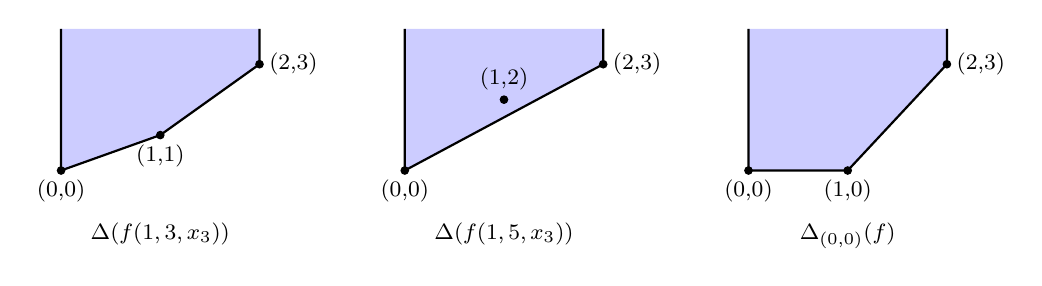
\begin{tikzpicture}[scale = 0.9, font = \footnotesize]
        \begin{scope}
        
        \fill[blue!20] (0,2) -- (0,0) -- (1.4,0.5) -- (2.8,1.5) -- (2.8,2);
        \draw[thick] (0,2) -- (0,0) -- (1.4,0.5) -- (2.8,1.5) -- (2.8,2);
        
        \filldraw[black] (0,0) circle (1.5pt) node[anchor=north] {(0,0)};
        \filldraw[black] (1.4,0.5) circle (1.5pt) node[anchor=north] {(1,1)};
        \filldraw[black] (2.8,1.5) circle (1.5pt) node[anchor=west] {(2,3)};

        \node[anchor = north] at (1.4,-0.6) {$\Delta(f(1,3,x_3))$};
        
        \end{scope}

        \begin{scope}[xshift = 4.85cm]
        
        \fill[blue!20] (0,2) -- (0,0) -- (2.8,1.5) -- (2.8,2);
        \draw[thick] (0,2) -- (0,0) -- (2.8,1.5) -- (2.8,2);
        
        \filldraw[black] (0,0) circle (1.5pt) node[anchor=north] {(0,0)};
        \filldraw[black] (1.4,1) circle (1.5pt) node[anchor=south] {(1,2)};
        \filldraw[black] (2.8,1.5) circle (1.5pt) node[anchor=west] {(2,3)};

        \node[anchor = north] at (1.4,-0.6) {$\Delta(f(1,5,x_3))$};

        
        \end{scope}
        
        \begin{scope}[xshift = 9.7cm]
        
        \fill[blue!20] (0,2) -- (0,0) -- (1.4,0) -- (2.8,1.5) -- (2.8,2);
        \draw[thick] (0,2) -- (0,0) -- (1.4,0) -- (2.8,1.5) -- (2.8,2);
        
        \filldraw[black] (0,0) circle (1.5pt) node[anchor=north] {(0,0)};
        \filldraw[black] (1.4,0) circle (1.5pt) node[anchor=north] {(1,0)};
        \filldraw[black] (2.8,1.5) circle (1.5pt) node[anchor=west] {(2,3)};

        \node[anchor = north] at (1.4,-0.6) {$\Delta_{(0,0)}(f)$};

        
        \end{scope}
    \end{tikzpicture}
    \caption{The expected Newton polygon and some possible Newton polygons of $f$ in Example \ref{ex:unique}.}
    \label{fig:unique}
\end{figure}


\subsection{Zero-dimensional Algorithm}
To keep things simple, we restrict ourselves to the task of computing just a single point on the tropical variety, as the algorithm's structure naturally extends to computing the entire tropical variety with appropriate bookkeeping.



\begin{algorithm}[\texttt{Tropical point, zero-dimensional case only}]\
  \begin{algorithmic}[1]
  \REQUIRE $F = \{f_1, \ldots,f_n\} \subseteq K[x_1,\ldots,x_n]$ a triangular set with \\\hspace{20pt}$V(\langle F \rangle) \subseteq (K^*)^n$.
  \ENSURE $w\in \trop\left(V(\langle F\rangle)\right)$
  \STATE Pick $w_1 \in \Lambda(f_1)$.
  \FOR{$i = 2,\ldots,n$}
    \IF{$f_i$ has a unique Newton polygon at $(w_1,\ldots, w_{i-1})$}
      \STATE Pick $w_i \in \Lambda_{(w_i,\ldots,w_{i-1})}(f_i)$.
    \ELSE
      \STATE Compute a root $(z_1,\ldots,z_{i-1}) \in V(f_1,\ldots,f_{i-1})$.
      \STATE Pick $w_i \in \Lambda(f_i(z_1,\ldots z_{i-1},x_i))$.
    \ENDIF
  \ENDFOR
  \RETURN{$(w_1,\ldots,w_n)$}
  \end{algorithmic}
  \label{alg:0Tropicalpoint}
\end{algorithm}

Let's breakdown Algorithm \ref{alg:0Tropicalpoint} step by step. So this algorithm takes a triangular set $F$ as the input, where the algebraic variety $V(F)$ consists of nontrivial solutions. The output of the algorithm is a point on the tropical variety $\trop(F)$. So we begin by computing the Newton polygon for the first polynomial in the triangular set $\Delta(f_1)$. We then pick $w_1 \in \Lambda(f_1)$, which is the set consisting of the negatives of the slopes admitted by $\Delta(f_1)$. The for loop in Step 2, loops through each remaining polynomial in the triangular set. If the polynomial $f_i$ has a unique Newton polygon at $(w_1,\ldots,w_{i-1})$ then we pick $w_i$ to be one of the negative slopes admitted by said Newton polygon. If $f_i$ does not have a unique Newton polygon at $(w_1,\ldots,w_{i-1})$ then we compute a solution $(z_1,\ldots,z_{i-1})$ of the algebraic variety of the previous polynomials $V(f_1,\ldots,f_{i-1})$. We then have the univariate polynomial $f_i(z_1,\ldots,z_{i-1},x_i)$, which has a unique Newton polygon. So we choose $w_i$ to be one of the negative slopes admitted by said Newton polygon. Finally, we then return the vector $w = (w_1,\ldots , w_n)$, which consists of all the choices of negative slopes.

\begin{figure}[t]
    \centering
    \includegraphics[width=\linewidth]{fig 3.png}
    \caption{A tree of unique Newton polygons. \cite{HR2018}}
    \label{fig:treeNewton}
\end{figure}

\begin{example}
So Algorithm \ref{alg:0Tropicalpoint} can be used to compute entire tropical varieties of zero-dimensional ideals by keeping track of all the choices of slopes. We begin by computing a triangular decomposition and applying the algorithm for each triangular set. Consider the triangular set $F = \{f_1, f_2, f_3\} \subseteq \QQ_p[x_1, x_2, x_3]$ with \[f_1 = px_1^2 + x_1  + 1, \quad f_2 = px_2^2 +x_1x_2 + 1, \quad f_3 = x_3+x_1x_2.\]
So working through the algorithm for this triangular set, we begin with constructing the Newton polygon of the univariate polynomial $f_1$, denoted by $\Delta(f_1)$. This Newton polygon then admits the two slopes $0$ and $1$, which we take the negative of, leaving us with the two choices $\Lambda(f_1) = \{0,-1\}$. For each choice of $w_1$, we take this value as the valuation of $x_1$, that is $\val(x_1) = w_1$, and construct the Newton polygon $\Delta_{(w_1)}(f_2)$. So here we have the two Newton polygons $\Delta_{(0)}(f_2)$ and $\Delta_{(-1)}(f_2)$. We then repeat this process taking the negative of the new slopes as the valuation of $x_2$ and evaluate the polynomial $f_3$ to construct the Newton polygons $\Delta_{(w_1,w_2)}(f_3)$. For example, one path of choices is $\Delta_{(-1,-2)}(f_3)$, which will have vertices $(0, -3)$ and $(1,0)$ and admit the slope $\Lambda_{(-1,-2)}(f_3) = \{-3\}$. So $F$ admits several choices of slopes throughout the algorithm, where each choice induces a unique Newton polygon, which can be seen in Figure \ref{fig:treeNewton}. Keeping track of all the choices of slopes, we can reconstruct the triangular set's entire tropical variety. Here we have: \[\trop(V(\langle F\rangle)) \; = \; \{(0,0,0), (0,-1,-1), (-1,1,0),(-1,-2,-3)\}\] 
\end{example}

\subsection{Computing Higher Dimensional Tropical  Points}\label{section:5}
We will now use Algorithm \ref{alg:0Tropicalpoint} to study \cite[Algorithm 3.2]{HR2018}, which computes points on higher dimensional tropical varieties. To do this we reduce the dimension to zero by intersecting the tropical variety with randomly chosen hyperplanes.

\begin{definition}
    (\cite[Def. 3.5.3]{GP2007}) Let $I \trianglelefteq K[x_1,\ldots,x_n]$ be an ideal. Then a subset \[u\subseteq x = \{x_1,\ldots,x_n\} \] is called an \textit{independent set} (with respect to $I$) if $I \cap K[u] = 0$. Furthermore, an independent set $u\subseteq x$ (with respect to $I$) is called \textit{maximal} if $\dim(K[x]/I) = \#u$. 
\end{definition}

\begin{algorithm}[\texttt{Tropical point}]\label{alg:Tropicalpoint}\
  \begin{algorithmic}[1] 
  \REQUIRE $I \trianglelefteq K[x_1,\ldots,x_n]$ prime ideal with $V(I) \cap(K^*)^n \neq \emptyset$.
  \ENSURE $w \in \trop(I)$
  \STATE Compute a maximal algebraically independent set modulo I, say \\$\{x_1,\ldots,x_d\}.$
  \REPEAT 
    \STATE Pick $z = (z_1, \ldots, z_d) \in (K^*)^d$ randomly
    \STATE Set $I_z$ to be the image of $I$ under the substitution map
    \[ K[x_1, \ldots, x_n] \rightarrow K[x_{d+1}, \ldots, x_n], \quad x_i \mapsto \begin{cases}
        z_i \text{ if } i \leq d,\\
        x_i \text{ else.}
    \end{cases}  \]
  \UNTIL dim($I_z) = 0$ and $V(I_z) \subseteq (K^*)^{n-d}$
  \STATE Compute a triangular set $F \subseteq K[x_{d+1}, \ldots, x_n]$ with $\sqrt{I_z} \subseteq \langle F\rangle$
  \STATE Compute a point $(w_{d+1}, \ldots, w_n) \in \trop(F)$ using Algorithm \ref{alg:0Tropicalpoint}.
  \RETURN{$(\nu(z), w_{d+1}, \ldots, w_n)$}
  \end{algorithmic}
\end{algorithm}
This algorithm takes as input, a prime ideal such that the algebraic variety has at least one solution, where none of the coordinates are zero. The ouput of the algorithm is a point on the tropical variety of the ideal. In Step 1, we begin by computing a maximal algebraically independent set modulo the ideal. In Steps 3 and 4, we take $I_z$ to be the image of $I$ under a substitution map that maps each variable in the maximal algebraically independent set to a random element in the field $K^*$. We repeat this process, each time with different randomly chosen values for each variable in the maximal algebraically independent set until we have a zero-dimensional ideal. Once we have a zero-dimensional ideal, we can then compute a triangular set for this ideal and use Algorithm \ref{alg:0Tropicalpoint} to compute a point in the tropical variety.


\section{Traversing Entire Tropical Varieties}
In this section we will study an algorithm  \cite[Algorithm 4.6]{HR2018} that computes links of a tropical variety around its one-codimensional Gröbner polyhedra. We do this in two main steps. Firstly, we intersect the link with a subspace to reduce it to a one-dimensional polyhedral fan. Then we intersect the link with random affine hyperplanes to determine all its rays.

\begin{definition}
    (\cite[Def. 4.1]{HR2018}) We refer to $\trop(V(I))$ as a tropical link, if it is a polyhedral fan and has a one-codimensional lineality space.
\end{definition}

\begin{algorithm}[\texttt{Tropical link}]\label{alg:Tropicallink}\
  \begin{algorithmic}[1] 
  \REQUIRE{$I \trianglelefteq K[x_1,\ldots,x_n]$ such that $\trop(I)$ is a $(d+1)$-dimensional tropical link with $d$-dimensional lineality space $H$.}
  \ENSURE{$W \subseteq \RR^n$ such that $\trop(I) = \bigcup_{w\in W}w\cdot\RR_{\geq 0} + H$}      
  \STATE Find $A \subseteq \{1,\ldots,n\}$ such that $|A| = n -d$ and $H \cap \text{Lin}(e_i \;| \; i \in A) = \{0\},$ say $A = \{d+1,\ldots, n\}$.
  \STATE Let $J$ be the image of $I$ under the substitution map
  \[ K[x_1, \ldots, x_n] \rightarrow K[x_d, \ldots, x_n], \quad x_i \mapsto \begin{cases}
      1 \text{ if } i < d,\\
      x_i \text{ else.}
  \end{cases}  \]
  \FOR{$i = d,\ldots,n$}
    \STATE Let $J_i^\pm$ be images of $J$ under the maps $x_i \mapsto p^{\pm 1}$ respectively.
    \IF{$J_i^\pm \neq \langle 1 \rangle$}
      \STATE Compute $T_i^\pm = \trop(J_i^\pm)$ using Algorithm \ref{alg:0Tropicalpoint}
      \STATE Set
      \begin{equation*}
      \begin{aligned}
          W_i^\pm := \{(0,\ldots,0,w_d, \ldots,w_{i-1},\pm1, w_{i+1},\ldots,w_n) &\in \RR^n \; | \\ \quad (w_d, \ldots,w_{i-1},w_{i+1},\ldots,w_n&) \in T_i^\pm\}.
      \end{aligned}
      \end{equation*}
      \STATE Scale elements of $W_i^\pm$ positively so that they are primitive in $\ZZ^n$.
    \ENDIF
  \ENDFOR
  \RETURN{$W:=\bigcup_{i=d}^nW_i^\pm$}
  \end{algorithmic}
\end{algorithm}
\vspace{5pt}
Algorithm \ref{alg:Tropicallink} takes as input an ideal such that the tropical variety of the ideal is a $(d+1)$-dimensional tropical link. This tropical link has a $d$-dimensional lineality space $H$, meaning it contains a $d$-dimensional space of directions in which it extends infinitely. The output of the algorithm is the subset of direction vectors $W$ such that the tropical variety is built up of the union of the rays extending in the directions of the elements of $W$. So in Step 1, we choose a subset $A \subseteq \{1,\ldots,n\}$ such that $A$ has $n-d$ elements. The second requirement on $A$ ensures that these directions are independent of the lineality space $H$. Then in Step 2, we compute the ideal $J$ by applying the substitution map to $I$, where each variable in the polynomial ring which is not in $A$, is mapped to $1$. This results in a one-dimensional tropical link with lineality space $\{0\}$. We then iterate over the variables in the polynomial ring of the ideal $J$ and for each $i$, we construct two new ideals $J_i^{\pm1}$, where we map the variable $x_i \mapsto p^{\pm1}$ respectively. Here, $p$ is the uniformiser of the valued field. This step is where we intersect the link with the affine hypersurfaces $\trop\left(V\langle x_i - p^{\pm1}\rangle \right)$ to reduce the ideal to a zero-dimensional ideal. Step 5 ensures that we ignore any trivial ideals since they do not contribute to the tropical variety. Now we have a zero-dimensional variety, we can use Algorithm \ref{alg:0Tropicalpoint} to compute the points in the tropical variety for the ideals $J_i^\pm$. We then construct the set of tropical points $W_i^\pm$, which consists of $n$-dimensional vectors whose first $d$ coordinates are $0$ as these coordinates are the variables that were fixed to 1 when we reduced the ideal to a one-dimensional ideal. The $i^{th}$ coordinate of the vectors in $W_i^{\pm1}$ is $\pm1$ respectively as this is the variable that was fixed to $p^{\pm1}$ and so applying the valuation map to this coordinate results in $\pm1$. The remaining coordinates come from $T_i^\pm$ in Step 6 where we computed the tropical points in the zero-dimensional tropical variety. Finally, we normalise the elements, ensuring that they are primitive elements in $\ZZ^n$. This essentially means that they are expressed in their simplest integer form. We then output the final set $W$, which is the union of all $W_i^\pm$.

The implementation of Algorithm \ref{alg:Tropicallink} in Julia using the {\sc oscar} algebra system can be found in Appendix \ref{apx:link} and in the GitHub repository \cite{LinksGitHub}.




\section{Optimisation Experiment - Key Variable Sets}
% Selecting a key variable subset 
% Explain how I am using heuristic methods to construct the subset greedily using the scoring function
% Change to an experiment, where we explain the experiment
% Exploring how to choose the key variable subset
% And then explain the results
In both Algorithm \ref{alg:Tropicalpoint} and Algorithm \ref{alg:Tropicallink}, we select a key variable subset to reduce the dimension of the ideal. In the tropical starting point algorithm we choose a maximal independent set and map these variables to random element of the field $K^*$ to reduce the dimension of the ideal to zero. In the tropical link algorithm, we take a key variable subset that has a trivial intersection with the lineality space of the ideal. 

\begin{contribution*}
In this section, I am going to plan and conduct an experiment to explore how to choose these key variable subsets. I will introduce algorithms that I have made that use scoring algorithms to carefully select which variables to include in the key variable subset. Then we will conclude by testing each key variable subset to see if the algorithms have helped choose an optimal subset for the given tasks. For the experiment involving the tropical link algorithm, which I implemented in {\sc oscar}, the framework and the relevant algorithms have been fully developed and explained in this section. However, testing and obtaining conclusive results were not possible, as the implementation of the tropical link algorithm depends on the \verb|tropical_variety| function, which is currently still under development within the {\sc oscar} system. The implementation of my experiment for both cases can be found in the Appendices \ref{apx:linkexperiment} and \ref{apx:pointexperiment} as well as the GitHub repository \cite{LinksGitHub}.

\end{contribution*}

\subsection{Tropical Link - Framework}
In the tropical link algorithm, we will have scoring algorithms that takes as input the index of a generator of the polynomial ring, that is $k \in [n]$. This scoring algorithm will then output a score for this variable $s_k \in \RR$.

\subsubsection*{Scoring Algorithms}
The first scoring algorithm is Algorithm \ref{alg:Degreecount} and will be a degree counting algorithm. 

\begin{algorithm}[\texttt{Degree count}]\label{alg:Degreecount}\
\begin{algorithmic}[1]
    \REQUIRE $I \trianglelefteq K[x_1,\ldots,x_n]$ and a variable $k \in [n]$.
    \ENSURE Score $s_k \in \RR$.
    \STATE $s_k = 0$
    \FOR{each $f = \sum_{\mathbf{u}=(u_1,\ldots,u_n)\in\NN^n}c_\mathbf{u}x^\mathbf{u} \in \text{Generators}(I)$}
    \FOR{each monomial $c_\mathbf{u}x^\mathbf{u} \in f$}
        \STATE $s_k = s_k + u_k$
    \ENDFOR
    \ENDFOR
    \RETURN $s_k$
\end{algorithmic}    
\end{algorithm}

This algorithm will compute a score for the variable $x_k$ using the generators of the ideal. It creates a counter variable, $s_k$, which is incremented by the degree of the variable $x_k$ in each monomial in each generator of the ideal. Then it returns this counter variable as the score for that variable.

The second scoring Algorithm \ref{alg:Initialdegreecount} is similar to the degree count algorithm. However, it will use the initial of the ideal to compute a score for the variable. 

\begin{algorithm}[\texttt{Initial Degree count}]\label{alg:Initialdegreecount}\
\begin{algorithmic}[1]
    \REQUIRE $I \trianglelefteq K[x_1,\ldots,x_n]$ with a weight vector $\mathbf{w}\in \Gamma_{\val}^n$ and a variable $k \in [n]$.
    \ENSURE Score $s_k \in \RR$.
    \STATE Compute the initial ideal $\initial_\mathbf{w}(I)$.
    \STATE $s_k = 0$
    \FOR{each $f = \sum_{\mathbf{u}=(u_1,\ldots,u_n)\in\NN^n}c_\mathbf{u}x^\mathbf{u} \in \text{Generators}(\initial_\mathbf{w}(I))$}
    \FOR{each monomial $c_\mathbf{u}x^\mathbf{u} \in f$}
        \STATE $s_k = s_k + u_k$
    \ENDFOR
    \ENDFOR
    \RETURN $s_k$
\end{algorithmic}    
\end{algorithm}

This algorithm requires a weight vector $\mathbf{w} \in \Gamma_{\val}^n$ as well as the index of the variable in the polynomial ring it is scoring $k\in[n]$. It begins by computing the initial of the ideal for the given weight vector and then initialises a counter variable $s_k$. Then the algorithm follows the degree counting algorithm; it increments the counter by the degree of the variable $x_k$ in each monomial in each generator of $\initial_\mathbf{w}(I)$. Finally, it returns this counter variable.

The difference between these two algorithms is the computation of the initial of the ideal. So the aim of this experiment is to evaluate whether the additional computational effort of computing the initial of the ideal results in a better selection of the key variable subset. 

\subsubsection*{Condition Algorithms}

We then have two simple algorithms that check the requirements of the key variable subset $A \subseteq [n]$. 

Algorithm \ref{alg:IsAadmissible} checks that the intersection of the lineality space of the ideal $H$ and the linear space generated by the standard basis vectors $e_i$ for $i\in A$ is trivial. The algorithm simply returns true if the intersection is trivial and false otherwise. 

\begin{algorithm}[\texttt{Lineality\_Check}] \label{alg:IsAadmissible}\
\begin{algorithmic}[1]
    \REQUIRE $I \trianglelefteq K[x_1,\ldots,x_n]$ such that $\trop(I)$ is a $(d+1)$-dimensional tropical link with $d$-dimensional lineality space $H$. A key variable subset $A \subseteq [n]$.
    \ENSURE true/false
    \IF{$H \cap\text{Lin}(e_i \; | \; i \in A) = \{0\}$}
        \RETURN true
    \ELSE
        \RETURN false
    \ENDIF
\end{algorithmic}    
\end{algorithm}

The second condition is to check if the subset is of the correct size. So Algorithm \ref{alg:IsAdone} simply returns true if the subset $A$ contains $n-d$ indices of variables in the polynomial ring, where $d$ is the dimension of the lineality space of the ideal. Otherwise, it returns false.

\begin{algorithm}[\texttt{Is\_A\_complete}]\label{alg:IsAdone}\
\begin{algorithmic}[1]
    \REQUIRE A key variable subset $A \subseteq [n]$.
    \ENSURE true/false
    \IF{$|A | = n - d$}
        \RETURN true
    \ELSE
        \RETURN false
    \ENDIF
\end{algorithmic}    
\end{algorithm}

These algorithms are simple, but crucial to ensure that we choose an appropriate key variable subset that follows the requirements stated in the tropical link algorithm.

\subsubsection*{Greedy Selection Algorithm}
The final algorithm for the experiment in the tropical link case is a greedy selection algorithm. This is the algorithm that will use the previous algorithms to actually select which variables to include in the subset.

\begin{algorithm}[\texttt{Greedy select}]\label{alg:Greedy}\
  \begin{algorithmic}[1]
  \REQUIRE $I \trianglelefteq K[x_1,\ldots,x_n]$ such that $\trop(I)$ is a $(d+1)$-dimensional tropical link with $d$-dimensional lineality space $H$. A scoring function \texttt{score}, and the condition functions \texttt{Lineality\_Check} and \texttt{Is\_A\_Complete}.
  \ENSURE A key variable subset $A$ such that $H \cap\text{Lin}(e_i \; | \; i \in A) = \{0\}$ and $|A| = n - d$.
  \STATE $A = \emptyset$
  \REPEAT
  \STATE $A = A \cup \argmin_{k \ \in \  [n]\setminus\Lambda,  \texttt{ Lineality\_Check}\left(I, \ A \cup \{k\}\right) = \text{true}} (\texttt{score}(k))$
  \UNTIL \texttt{Is\_A\_Complete(A)}
  \RETURN $A$
  \end{algorithmic}
\end{algorithm}

Algorithm \ref{alg:Greedy} takes as input the ideal, one of the two scoring algorithms and the two condition algorithms. The output of the algorithm is the subset of key variables $A$ that follows the two requirements necessary for the tropical link Algorithm \ref{alg:Tropicallink}. We begin in Step 1, by initialising the subset as an empty set. We then initialise a loop that repeats until the subset is of size $n-d$, and we use Algorithm \ref{alg:IsAdone} to check this. Within this loop, we select the indices of the variables one by one. We do this by taking the index of the variable; that isn't already included in the subset, that has the lowest score and satisfies the \texttt{Lineality\_Check} algorithm. This ensures we don't have any repeated variables in the subset. Then once the subset $A$ is of the correct size, we return the subset.

\subsection{Tropical Point - Framework}
In the tropical starting point algorithm, the aim of the task is to compute a maximal algebraically independent set modulo the ideal, so that we can map the variables in the set to a random element of the field, ultimately reducing the ideal to dimension 0. This means that the framework of this experiment will vary a little from the previous case. Previously, we scored each variable in the polynomial ring and then chose the subset based on this score. Here, we will compute all maximal independent sets and then assign a score to each set rather than the individual variables. This means that there is no need for a greedy selection algorithm or algorithms that check that the subset meets the requirements necessary for Algorithm \ref{alg:Tropicalpoint}.

\subsubsection*{Scoring Algorithm}
So Algorithm \ref{alg:independentscore}, is our scoring algorithm for this experiment. This algorithm again is just a degree counting algorithm, that counts the degrees of the variables as they appear in the generators of the ideal. However, we now do this for all the variables in the independent set, this can be seen in the for loop on line 2 of the algorithm.

\begin{algorithm}[\texttt{Independent Set Score}]\label{alg:independentscore}\
\begin{algorithmic}[1]
    \REQUIRE $I \trianglelefteq K[x_1,\ldots,x_n]$ prime ideal with $V(I) \cap(K^*)^n \neq \emptyset$ and a maximal algebraically independent set modulo $I$, say $\{x_1,\ldots,x_d\}$. 
    \ENSURE A score for the set, denoted $s \in \RR$.
    \STATE $s = 0$
    \FOR{each $x_k \in \{x_1,\ldots,x_d\}$}
    \FOR{each $f = \sum_{\mathbf{u}=(u_1,\ldots,u_n)\in\NN^n}c_\mathbf{u}x^\mathbf{u} \in \text{Generators}(I)$}
    \FOR{each monomial $c_\mathbf{u}x^\mathbf{u} \in f$}
        \STATE $s = s + u_k$
    \ENDFOR
    \ENDFOR
    \ENDFOR
    \RETURN score
\end{algorithmic}    
\end{algorithm}

\subsection*{Tropical Point - Testing}
Now that we have established a method to score a maximal algebraically independent set, we now need to test whether this scoring algorithm has helped to optimise the tropical starting point Algorithm \ref{alg:Tropicalpoint}.

So we shall begin by randomly generating an ideal $I$, with $\text{dim}(I) \geq 0$. Then for each maximal algebraically independent set modulo $I$, we will construct the map in Step 2 of Algorithm \ref{alg:Tropicalpoint}. This is the map that fixes the variables in the independent set to a random element in the field with the aim of reducing the ideal to a 0-dimensional ideal. So now we have a 0-dimensional ideal, we will use the {\sc oscar} function \verb|triangular_decomposition| to compute a triangular decomposition of the ideal. We will compare the time taken to compute the triangular set for each given independent set and see the correlation between the score of the set and the computation time. We expect to see that as the scores of the sets increase, the computation time when computing the triangular decomposition will decrease.


\subsection{Tropical Point - Results Discussion}

To assess the effectiveness of the degree count scoring heuristic on the tropical starting point algorithm, I attempted to construct a series of randomly generated ideals. The motivation here was to observe whether the heuristic score correlated with the computational difficulty of performing a triangular decomposition, particularly in terms of the Gröbner basis computation involved.

This procedure involved generating random ideals in polynomial rings with a specified number of variables, generators, and the degree of the generators. Once this ideal had been constructed, I applied a transformation to the ideal that ``inflated" the exponents of certain randomly selected variables by raising them to higher powers. This was intended to create a variation in the heuristic scores for the independent sets, allowing us to observe and test if there was a difference in computation time. By testing ideals with a wide range of the various parameters; including the field, number of variables, number of generators, degree of the generators, and the inflation factor, I hoped to obtain a varied collection of ideals for which I would evaluate the scoring algorithm.

However, the results were ultimately inconclusive. After reducing the ideals to 0-dimensional ideals, the triangular decomposition function either completed almost instantaneously or stalled indefinitely during the Gröbner basis computation step. Despite testing a wide range of parameters, the majority of generated ideals turned out to be trivially decomposable or extremely difficult to handle, often due to high degrees. Additionally, while the inflation process successfully created varied heuristic scores, it did not reliably increase the computational difficulty in a measurable way. This led to highly inconsistent behaviour and prevented a meaningful correlation from being observed between the heuristics scores and the computation effort. The results of an ideal where the triangular decomposition was computed almost instantaneously, can be seen in Figure \ref{fig:results}. It is clear that these computed too fast and the choice of independent set did not have an effect. Therefore, we were unable to evaluate the effectiveness of the heuristic scoring algorithm.

\begin{figure}
    \centering
    \includegraphics[width=0.75\linewidth]{Scatter graph.png}
    \caption{The score of the independent set against the computation time of the triangular decomposition}
    \label{fig:results}
\end{figure}


For these reasons, I was unable to obtain a consistent or informative dataset to test the heuristic algorithm meaningfully. However, this experiment helped to clarify the challenges involved in evaluating variable heuristics using randomly generated ideals and highlighted the need for more structured or purpose-built test cases.



\section{Conclusion}
In this report, we have introduced the key structures and definitions underpinning tropical algebra and geometry, with a particular focus on the computation of tropical varieties. To support this, we examined several fundamental geometric and algebraic tools that form the building blocks of tropical geometry. These included Newton polytopes, which encode combinatorial information for polynomials; polyhedral geometry, which provided definitions for the structures of tropical varieties; and initial forms, which allowed us to bridge classical and tropical algebra through valuation maps. Furthermore, by studying and reimplementing algorithms for computing tropical points and tropical links in Julia with the {\sc oscar} system, we demonstrated the practical feasibility of tropical computations. 

In the final chapter, we included an optimisation experiment that explored how heuristic methods can influence the performance of the algorithm. Although no concrete results were obtained, this experiment highlighted that future work could focus on refining these heuristics, improving computational efficiency, and applying these methods to broader classes of ideals. Overall, this project contributes to the algorithmic side of tropical geometry and lays the foundation for continued development in the computational aspects of tropical geometry.

% 2 optimisations
% 1. Generators
% WE want minimal degree left in A 


% 2. Weighting of the initial of the ideal
% Heuristic algorithm given the weight values for the monomials

% After implemented optimisations we can construct examples
% Random ideal, random weight vector 


% Computing all cycles of the lex GB 
\newpage
\printbibliography
\newpage
\begin{appendices}
The code in the following appendices was written using Visual Studio Code. During development, GitHub Copilot \cite{GitHub_Copilot} was used to assist with code completion and suggestions. All of the following code can be found in the following GitHub repository \cite{LinksGitHub} along with a README file that explains the functions.
\section{Tropical Link Implementation} \label{apx:link}
\inputminted[breaklines, breakanywhere, style = friendly, baselinestretch=1.2, fontsize = \small, linenos]{julia}{tropical_link_functions.jl}

\section{Tropical Link Experiment} \label{apx:linkexperiment}
\inputminted[breaklines, breakanywhere, style = friendly, baselinestretch=1.2, fontsize = \small, linenos]{julia}{tropical_link_experiment_functions.jl}

\section{Tropical Point Experiment} \label{apx:pointexperiment}
\inputminted[breaklines, breakanywhere, style = friendly, baselinestretch=1.2, fontsize = \small, linenos]{julia}{tropical_point_experiment_functions.jl}
\end{appendices}
\end{document}